\documentclass[a4paper,12pt]{report}
\usepackage[utf8]{vietnam}
\usepackage{graphicx}
\usepackage{hyperref}
\usepackage{amsmath, amssymb}
\usepackage{geometry}
\usepackage{subcaption}
\usepackage{float} % để dùng [H]
\usepackage{fancyhdr} % Thêm gói fancyhdr để tùy chỉnh header
\usepackage{xcolor} % Để sử dụng màu xanh cho chữ

% Thiết lập kích thước header trước khi định nghĩa geometry
\setlength{\headheight}{45pt}

% Điều chỉnh lề, đặc biệt là lề trên cao hơn để tránh chồng lấn
\geometry{left=3cm, right=2.5cm, top=4cm, bottom=2.5cm, headheight=45pt, headsep=0.5cm}

\usepackage{tikz}
\usetikzlibrary{arrows.meta, positioning}

% Định nghĩa kiểu header
\fancypagestyle{reportstyle}{
  \fancyhf{} % Xóa tất cả header và footer hiện tại
  \fancyhead[L]{%
    
\includegraphics[height=1.5cm]{latex/imgs/logoITSGU.png}
    \hspace{0.5cm}
    \begin{minipage}[b]{0.7\textwidth}
      {\color{blue}\textbf{Trường Đại học Sài Gòn}}\\
      {\color{blue}\textbf{Khoa Công Nghệ Thông Tin}}
    \end{minipage}
  }
  \renewcommand{\headrulewidth}{0.4pt} % Đường kẻ phía dưới header
  \fancyfoot[C]{\thepage} % Thêm số trang ở giữa footer
}

% Thiết lập pagestyle mặc định cho toàn bộ tài liệu
\pagestyle{reportstyle}

% Đảm bảo header xuất hiện trên tất cả các trang chapter
\makeatletter
\renewcommand{\chapter}{\if@openright\cleardoublepage\else\clearpage\fi
  \thispagestyle{reportstyle}% Áp dụng header cho trang đầu của chapter
  \global\@topnum\z@
  \@afterindentfalse
  \secdef\@chapter\@schapter}
\makeatother

\begin{document}
% === TRANG BÌA ===
\begin{titlepage}
    \thispagestyle{empty} % Không hiển thị header trên trang bìa
    \centering
    
\includegraphics[width=4cm]{latex/imgs/logoITSGU.png} \\[1cm]
    \textbf{\Large TRƯỜNG ĐẠI HỌC SÀI GÒN} \\[0.5cm]
    \textbf{\Large KHOA CÔNG NGHỆ THÔNG TIN} \\[2cm]
    {\Huge \textbf{BÁO CÁO ĐỒ ÁN}} \\[2cm]
    \begin{center}
        \begin{tabular}{|c|c|c|c|}
            \hline
            \textbf{Họ và tên sinh viên} & \textbf{Mã số sinh viên} & \textbf{Lớp} & \textbf{Email} \\
            \hline
            Trần Công Nguyên & 3121410352 & DCT1212 & nguyennrdz@gmail.com \\
            \hline
            Trần Thị Thủy & 3121410487 & DCT1218 & tranthithuy1375@gmail.com \\
            \hline
            Nguyễn Minh Quang & 3121560008 & DKP1211 & minhquangnmq11@gmail.com \\
            \hline
            Nguyễn Minh Phi & 3121560067 & DKP1211 & nmphi2710@gmail.com \\
            \hline
            Phan Thị Anh Thư & 3121410490 & DCT1212 & anhthu115599@gmail.com \\
            \hline
        \end{tabular}
        
    \end{center}
    
    \vspace{1cm}
    \textbf{Giảng viên hướng dẫn:} Từ Lãng Phiêu \\
    \vfill
    TP. Hồ Chí Minh, \today
\end{titlepage}

% Đảm bảo mục lục cũng có header
\pagenumbering{roman} % Sử dụng số La Mã cho mục lục
\tableofcontents
\cleardoublepage

% Bắt đầu đánh số trang bằng số Ả Rập từ chapter 1
\pagenumbering{arabic}
% Các chapter
\chapter{Giới thiệu đề tài}

\section{Lý do chọn đề tài}

Trong kỷ nguyên công nghệ số phát triển mạnh mẽ như hiện nay, âm nhạc trực tuyến không chỉ là một hình thức giải trí phổ biến mà còn là một phần thiết yếu trong đời sống tinh thần của con người. Với sự bùng nổ của các nền tảng âm nhạc trực tuyến như Spotify, Apple Music, hay Zing MP3, người dùng ngày càng quen thuộc với việc nghe nhạc mọi lúc, mọi nơi, trên mọi thiết bị. Những nền tảng này không chỉ cung cấp thư viện nhạc khổng lồ, mà còn tích hợp các công nghệ tiên tiến như trí tuệ nhân tạo (AI) để cá nhân hoá trải nghiệm người nghe.

Chính vì vậy, nhóm quyết định lựa chọn đề tài xây dựng hệ thống API mô phỏng nền tảng nghe nhạc trực tuyến – lấy cảm hứng từ Spotify – nhằm khám phá và ứng dụng những công nghệ hiện đại trong việc xây dựng một hệ thống backend thực tế. Đề tài này không chỉ giúp nhóm nâng cao kiến thức về thiết kế hệ thống, mà còn tạo điều kiện để rèn luyện các kỹ năng mềm trong môi trường làm việc nhóm.

Cụ thể, đề tài hướng đến các mục tiêu sau:
\begin{itemize}
    \item Tìm hiểu và áp dụng các công nghệ hiện đại như Django REST Framework, MongoDB, Postman, Docker, v.v.
    \item Thiết kế và phát triển một hệ thống API có khả năng mô phỏng các chức năng cơ bản của một ứng dụng nghe nhạc: đăng ký, đăng nhập, phát nhạc, tạo và quản lý danh sách phát.
    \item Rèn luyện kỹ năng lập trình backend, thiết kế cơ sở dữ liệu NoSQL và triển khai API theo kiến trúc RESTful.
    \item Nâng cao tinh thần làm việc nhóm, khả năng tổ chức và quản lý dự án, đặc biệt là trong môi trường mô phỏng thực tế.
\end{itemize}

\section{Bối cảnh thực hiện}

Đề tài được thực hiện trong khuôn khổ môn học \textbf{Hệ điều hành}, thuộc chương trình đào tạo ngành Công nghệ Thông tin tại \textbf{Trường Đại học Sài Gòn}. Trong học phần này, sinh viên được yêu cầu áp dụng tổng hợp các kiến thức lý thuyết và kỹ năng lập trình đã học để xây dựng một hệ thống có tính ứng dụng thực tế.

Với mong muốn kết nối lý thuyết và thực hành, nhóm quyết định chọn đề tài xây dựng hệ thống backend API phục vụ một ứng dụng âm nhạc trực tuyến, xem đây như một bước đệm để tiếp cận các dự án thực tế trong tương lai.

\begin{itemize}
    \item \textbf{Thời gian thực hiện}: Trong học kỳ II năm học 2024–2025.
    \item \textbf{Địa điểm}: Phòng thực hành Công nghệ Thông tin, Trường Đại học Sài Gòn.
    \item \textbf{Công cụ sử dụng}: Django REST Framework, MongoDB, Postman, GitHub, Docker, VS Code.
    \item \textbf{Phạm vi}: Tập trung phát triển hệ thống backend API ổn định, bảo mật và sẵn sàng mở rộng; frontend sẽ được đề cập trong giai đoạn sau.
\end{itemize}

\section{Mục tiêu của đề tài}

Đề tài hướng đến việc xây dựng một hệ thống backend mạnh mẽ, có khả năng mô phỏng trải nghiệm cơ bản của người dùng trên nền tảng âm nhạc trực tuyến. Các mục tiêu cụ thể bao gồm:

\begin{itemize}
    \item Xây dựng hệ thống RESTful API phục vụ các chức năng: xác thực người dùng, phát nhạc, quản lý danh sách phát.
    \item Thiết kế cơ sở dữ liệu sử dụng MongoDB, đảm bảo dữ liệu được tổ chức hợp lý và dễ truy vấn.
    \item Bảo mật hệ thống bằng cách tích hợp JWT (JSON Web Token) trong quá trình xác thực người dùng.
    \item Viết tài liệu hướng dẫn sử dụng API, giúp các lập trình viên frontend có thể tích hợp hệ thống một cách thuận tiện.
    \item Đảm bảo tính mở rộng và dễ bảo trì của hệ thống, hướng đến khả năng phát triển lâu dài.
\end{itemize}

\section{Ý nghĩa thực tiễn}

Đề tài mang lại nhiều giá trị thực tiễn, không chỉ ở khía cạnh học thuật mà còn cả kỹ năng nghề nghiệp:

\begin{itemize}
    \item Giúp sinh viên tiếp cận quy trình phát triển một hệ thống backend API thực tế, từ khâu thiết kế, lập trình đến triển khai.
    \item Là bước đệm quan trọng cho các dự án lớn hơn trong tương lai, đặc biệt là các hệ thống dịch vụ số liên quan đến âm nhạc, video hoặc nội dung số khác.
    \item Tài liệu và mã nguồn của đề tài có thể trở thành nguồn tham khảo hữu ích cho các bạn sinh viên khác trong các học phần liên quan đến lập trình backend, phát triển API hoặc quản lý dữ liệu NoSQL.
    \item Nâng cao kỹ năng giải quyết vấn đề, tư duy logic, làm việc nhóm và tinh thần tự học – những yếu tố quan trọng trong nghề nghiệp lập trình.
\end{itemize}

\chapter{Cơ sở lý thuyết}
\section{Thư viện và công nghệ sử dụng}
\subsection{API}

Phần API trong hệ thống đóng vai trò là tầng trung gian giữa cơ sở dữ liệu và giao diện người dùng, thực hiện xử lý logic nghiệp vụ và cung cấp dữ liệu thông qua các endpoint RESTful. Việc thiết kế API dựa trên mô hình client-server giúp tách biệt phần backend và frontend, cho phép phát triển độc lập, mở rộng dễ dàng, và tăng tính bảo trì cho hệ thống. Dưới đây là các công nghệ và thư viện chính đã được sử dụng trong việc xây dựng API:

\begin{itemize}

    \item \textbf{Django}: 
    Django là một framework phát triển web mã nguồn mở được viết bằng ngôn ngữ Python, tuân theo triết lý ``Don't Repeat Yourself (DRY)'' và mô hình kiến trúc \textit{Model-View-Template (MVT)}. Django được thiết kế để giúp các lập trình viên phát triển ứng dụng nhanh chóng và an toàn. Một số tính năng nổi bật của Django bao gồm:
    \begin{itemize}
        \item \textit{ORM (Object-Relational Mapping)}: Cho phép ánh xạ các lớp Python thành bảng trong cơ sở dữ liệu quan hệ, giúp thao tác với dữ liệu bằng Python thay vì SQL thuần.
        \item \textit{Hệ thống authentication và authorization}: Django tích hợp sẵn mô hình người dùng, hệ thống phân quyền, bảo vệ dữ liệu người dùng.
        \item \textit{Hệ thống middleware}: Hỗ trợ xử lý các yêu cầu và phản hồi HTTP, tích hợp xác thực, logging, và các chức năng bảo mật như CSRF protection.
        \item \textit{Quản lý routing bằng URLconf}: Cho phép định tuyến URL tới các view tương ứng một cách rõ ràng và linh hoạt.
        \item \textit{Admin interface mạnh mẽ}: Giao diện quản trị tự động sinh từ các mô hình dữ liệu, giúp quản lý nội dung dễ dàng.
    \end{itemize}

    \item \textbf{Django REST Framework (DRF)}:
    Là một thư viện mở rộng mạnh mẽ của Django giúp xây dựng các API RESTful một cách hiệu quả. DRF trừu tượng hóa các thao tác với dữ liệu thông qua các lớp như \textit{Serializers}, \textit{Views}, và \textit{ViewSets}. Những tính năng nổi bật của DRF bao gồm:
    \begin{itemize}
        \item \textit{Serializers}: Chuyển đổi dữ liệu giữa dạng đối tượng Python và JSON/XML khi trao đổi qua HTTP.
        \item \textit{Generic Views / ViewSets / Routers}: Hỗ trợ định nghĩa các endpoint CRUD nhanh chóng chỉ với vài dòng code.
        \item \textit{Hệ thống xác thực}: Tích hợp sẵn các phương thức xác thực như Token, JWT, OAuth2, Session.
        \item \textit{Giao diện web test API}: Giao diện trực quan giúp kiểm thử và quan sát dữ liệu trả về từ endpoint dễ dàng.
        \item \textit{Pagination, Filtering, Throttling}: Hỗ trợ phân trang, lọc dữ liệu và giới hạn tốc độ truy cập để nâng cao hiệu suất.
    \end{itemize}

    \item \textbf{MongoEngine}:
    Là thư viện \textit{Object-Document Mapper (ODM)} dành cho MongoDB. Thay vì làm việc với tài liệu BSON trực tiếp, MongoEngine cho phép định nghĩa các mô hình Python tương tự Django ORM, giúp thao tác với MongoDB dễ dàng và trực quan hơn. Các đặc điểm chính:
    \begin{itemize}
        \item Cho phép ánh xạ cấu trúc tài liệu MongoDB vào các lớp Python.
        \item Hỗ trợ quan hệ giữa các tài liệu bằng kỹ thuật Reference và Embedded Document.
        \item Tương thích tốt với Django khi cấu hình chính xác.
    \end{itemize}

    \item \textbf{Django CORS Headers}:
    Đây là thư viện mở rộng giúp xử lý chính sách \textit{Cross-Origin Resource Sharing (CORS)} trong Django. Trong một hệ thống có frontend và backend tách rời (ví dụ: Angular ở cổng 4200, Django ở cổng 8000), trình duyệt sẽ chặn các yêu cầu không cùng nguồn (cross-origin) nếu không được cho phép. Django CORS Headers giúp cấu hình các domain nào được phép truy cập API Django, từ đó tránh lỗi CORS Policy.
    
    \item \textbf{Daphne}:
    Daphne là một máy chủ ứng dụng tương thích với chuẩn ASGI (Asynchronous Server Gateway Interface), được thiết kế để thay thế WSGI trong các ứng dụng cần giao tiếp bất đồng bộ như WebSocket hoặc các luồng realtime. Daphne là thành phần chính trong bộ Channels Stack, cho phép ứng dụng Django xử lý đồng thời nhiều kết nối bất đồng bộ, thích hợp cho các ứng dụng chat, livestream,...

    \item \textbf{Channels}:
    Channels mở rộng lõi đồng bộ của Django để hỗ trợ các giao thức bất đồng bộ như WebSocket, HTTP/2 hoặc các tác vụ nền. Channels sử dụng các thành phần như:
    \begin{itemize}
        \item \textit{Consumers}: Đóng vai trò tương tự như Views nhưng cho WebSocket, có thể xử lý các sự kiện kết nối, nhận, gửi dữ liệu.
        \item \textit{Channel Layer}: Lớp truyền thông cho phép các tiến trình giao tiếp với nhau thông qua hàng đợi.
        \item \textit{Redis}: Thường được dùng làm backend cho Channel Layer để đồng bộ dữ liệu giữa các tiến trình.
    \end{itemize}
    Việc tích hợp Channels giúp API có thể giao tiếp realtime với client mà không cần tải lại trang, ví dụ như hiển thị tin nhắn, thông báo,...

    \item \textbf{PyMongo}:
    PyMongo là thư viện chính thức từ MongoDB, dùng để thao tác với cơ sở dữ liệu MongoDB thông qua Python. Không giống MongoEngine, PyMongo làm việc trực tiếp với các tài liệu BSON, cho hiệu năng cao hơn và kiểm soát chặt hơn trong các truy vấn nâng cao. Các tính năng của PyMongo bao gồm:
    \begin{itemize}
        \item Kết nối tới MongoDB server qua URI, xác thực, và cấu hình SSL.
        \item Hỗ trợ truy vấn nâng cao, aggregation pipelines, index và thao tác tập hợp dữ liệu.
        \item Là thư viện chuẩn dùng trong các tác vụ có hiệu năng yêu cầu cao, hoặc xử lý dữ liệu phức tạp.
    \end{itemize}

\end{itemize}


\subsection{Frontend}

Phần frontend của ứng dụng đóng vai trò xây dựng giao diện người dùng (User Interface - UI) và tương tác trực tiếp với người dùng cuối. Tầng này được phát triển bằng các công nghệ hiện đại, đảm bảo hiệu suất cao, dễ bảo trì, đồng thời mang lại trải nghiệm người dùng trực quan và thân thiện. Dưới đây là các công nghệ chính được sử dụng:

\begin{itemize}

    \item \textbf{Angular}:
    Angular là một framework mã nguồn mở do Google phát triển, sử dụng ngôn ngữ TypeScript để xây dựng các ứng dụng web đơn trang (Single Page Application - SPA). Angular sử dụng kiến trúc \textit{Component-Based}, giúp tách biệt từng phần giao diện thành các module nhỏ, dễ dàng tái sử dụng và kiểm thử. Các tính năng chính bao gồm:
    \begin{itemize}
        \item \textit{Data Binding}: Hỗ trợ liên kết dữ liệu hai chiều (two-way binding) giữa giao diện và logic.
        \item \textit{Dependency Injection}: Cho phép quản lý và tái sử dụng các dịch vụ, giảm sự phụ thuộc giữa các thành phần.
        \item \textit{Routing Module}: Hỗ trợ chuyển đổi giữa các trang trong SPA mà không cần tải lại trang.
        \item \textit{Forms (Template-driven và Reactive Forms)}: Cho phép xây dựng các biểu mẫu linh hoạt, có kiểm tra và xác thực dữ liệu.
    \end{itemize}
    Trong đồ án này, Angular được sử dụng để xây dựng các thành phần giao diện như quản lý bài hát, album, danh sách phát và tính năng phát nhạc trực tuyến.

    \item \textbf{Tailwind CSS}:
    Tailwind CSS là một CSS framework dạng \textit{utility-first}, cung cấp các lớp tiện ích sẵn có để xây dựng giao diện mà không cần viết CSS thuần. Việc sử dụng Tailwind giúp:
    \begin{itemize}
        \item Tăng tốc quá trình thiết kế giao diện nhờ các lớp tiện ích sẵn.
        \item Đảm bảo giao diện đồng nhất, hiện đại và dễ tùy biến.
        \item Loại bỏ tình trạng CSS trùng lặp nhờ cơ chế tree-shaking tích hợp với build tool như Vite hoặc Webpack.
    \end{itemize}
    Trong ứng dụng, Tailwind CSS được sử dụng để thiết kế các thành phần như bảng dữ liệu, nút điều khiển, layout chính, form nhập liệu và phần phát nhạc.

    \item \textbf{RxJS (Reactive Extensions for JavaScript)}:
    RxJS là một thư viện lập trình phản ứng (reactive programming) dựa trên luồng dữ liệu bất đồng bộ (asynchronous data streams). Angular tích hợp sâu với RxJS thông qua \texttt{Observable}, giúp:
    \begin{itemize}
        \item Quản lý dữ liệu từ API một cách linh hoạt.
        \item Đồng bộ hóa trạng thái ứng dụng theo thời gian thực.
        \item Xử lý các thao tác bất đồng bộ như HTTP request, WebSocket, sự kiện DOM.
    \end{itemize}
    Việc sử dụng RxJS giúp frontend hoạt động hiệu quả trong việc cập nhật dữ liệu liên tục mà không gây tải lại trang.

    \item \textbf{TypeScript}:
    TypeScript là một siêu ngôn ngữ của JavaScript, bổ sung hệ thống kiểu tĩnh (static typing) cùng với các tính năng hướng đối tượng mạnh mẽ. Những ưu điểm của TypeScript bao gồm:
    \begin{itemize}
        \item Dễ phát hiện lỗi tại thời điểm biên dịch (compile-time).
        \item Hỗ trợ kiểm tra và gợi ý thông minh từ trình soạn thảo (IntelliSense).
        \item Dễ bảo trì và mở rộng hệ thống nhờ tính rõ ràng của mã nguồn.
    \end{itemize}
    Trong đồ án, toàn bộ mã nguồn frontend được phát triển bằng TypeScript để đảm bảo độ ổn định, khả năng kiểm soát logic ứng dụng và dễ dàng bảo trì trong các giai đoạn nâng cấp sau này.

\end{itemize}


\section{Cấu trúc mã nguồn}
\subsection{API}
Cấu trúc thư mục chính của phần API được tổ chức như sau:
\begin{itemize}
    \item \textbf{spotify-api/}: Thư mục chính chứa mã nguồn API.
    \begin{itemize}
        \item \textbf{settings.py}: File cấu hình chính của Django, chứa các thông tin như cấu hình cơ sở dữ liệu, ứng dụng cài đặt, và các thông số bảo mật.
        \item \textbf{urls.py}: File định tuyến URL, ánh xạ các endpoint API đến các view tương ứng.
        \item \textbf{models.py}: File định nghĩa các mô hình dữ liệu, bao gồm các bảng và quan hệ trong cơ sở dữ liệu.
        \item \textbf{views.py}: File xử lý logic cho các endpoint API, bao gồm các chức năng như đăng ký, đăng nhập, và quản lý người dùng.
        \item \textbf{serializers.py}: File chuyển đổi dữ liệu giữa mô hình Python và định dạng JSON để giao tiếp với frontend.
    \end{itemize}
    \item \textbf{requirements.txt}: File liệt kê các thư viện cần thiết để chạy API, giúp dễ dàng cài đặt môi trường phát triển.
\end{itemize}

\subsection{Frontend}
Cấu trúc thư mục chính của phần frontend được tổ chức như sau:
\begin{itemize}
    \item \textbf{src/}: Thư mục chính chứa mã nguồn Angular.
    \begin{itemize}
        \item \textbf{app/}: Chứa các component và service chính
        \begin{itemize}
            \item \textbf{admin/}: Chứa các component quản trị như \texttt{admin-dashboard-management}, \texttt{admin-user-management}, \texttt{admin-album-management}, \texttt{admin-songs-management}, \texttt{admin-artist-management}.
            \item \textbf{shared/}: Chứa các component dùng chung như \texttt{toast-message}.
            \item \textbf{services/}: Chứa các service như \texttt{login.service.ts}, \texttt{songs.service.ts}, \texttt{artists.service.ts}.
            \item \textbf{components khác}: Các component chính như \texttt{profile}, \texttt{my-play-list}, \texttt{album}, \texttt{detail}, \texttt{login}, \texttt{register}, \texttt{video}.
        \end{itemize}
        \item \textbf{assets/}: Chứa các tài nguyên như hình ảnh (\texttt{Img/}), file CSS, và các tài nguyên tĩnh khác.
        \item \textbf{environments/}: Chứa cấu hình môi trường (\texttt{environment.ts} cho dev, \texttt{environment.prod.ts} cho production).
    \end{itemize}
    \item \textbf{angular.json}: File cấu hình dự án Angular, định nghĩa các thông số build, serve, và cấu trúc dự án.
    \item \textbf{package.json}: Danh sách các thư viện cần thiết cho frontend, bao gồm các dependency như \texttt{@angular/core}, \texttt{rxjs}, \texttt{tailwindcss}.
    \item \textbf{tailwind.config.js}: File cấu hình Tailwind CSS, định nghĩa các lớp utility được sử dụng trong dự án.
\end{itemize}

\section{Mô hình ứng dụng và các tính năng}
\subsection{Mô hình tổng thể}
Hệ thống được xây dựng theo mô hình \textbf{client-server}, trong đó hai thành phần chính là \textbf{Backend API} và \textbf{Frontend} phối hợp chặt chẽ để cung cấp các chức năng của ứng dụng. 

\textbf{Phần Backend API} chịu trách nhiệm xử lý toàn bộ logic nghiệp vụ, xác thực người dùng, và quản lý dữ liệu. API được xây dựng trên nền tảng \textbf{Django REST Framework (DRF)}, sử dụng cơ sở dữ liệu \textbf{MongoDB} để lưu trữ thông tin như người dùng, bài hát, danh sách phát, và các dữ liệu liên quan. Backend API cung cấp các endpoint RESTful để frontend có thể giao tiếp, đảm bảo tính bảo mật và hiệu suất cao.

\textbf{Phần Frontend} được phát triển bằng \textbf{Angular}, cung cấp giao diện người dùng hiện đại, thân thiện và dễ sử dụng. Frontend chịu trách nhiệm hiển thị dữ liệu từ API, đồng thời cho phép người dùng thực hiện các thao tác như đăng ký, đăng nhập, tìm kiếm bài hát, quản lý danh sách phát, và phát nhạc trực tuyến. Giao tiếp giữa frontend và backend được thực hiện thông qua các yêu cầu HTTP với dữ liệu được trao đổi dưới định dạng JSON.

Mô hình này đảm bảo tính phân tách rõ ràng giữa giao diện người dùng và logic xử lý phía server, giúp hệ thống dễ dàng mở rộng, bảo trì và tích hợp thêm các tính năng mới trong tương lai.

\subsection{Các tính năng được xây dựng}
Hệ thống được thiết kế và phát triển với các tính năng chính, bao gồm cả phần \textbf{API} và \textbf{Frontend}, nhằm đáp ứng nhu cầu quản lý và phát nhạc trực tuyến.

\begin{itemize}
    \item \textbf{Đăng ký và đăng nhập người dùng}:
    \begin{itemize}
        \item Cho phép người dùng tạo tài khoản mới và đăng nhập vào hệ thống.
        \item Hỗ trợ xác thực thông qua email và mật khẩu.
    \end{itemize}
    \item \textbf{Xác thực và phân quyền người dùng}:
    \begin{itemize}
        \item Sử dụng token để xác thực người dùng, đảm bảo chỉ những người dùng hợp lệ mới có thể truy cập các tài nguyên.
        \item Phân quyền người dùng dựa trên vai trò (admin, user) để kiểm soát quyền truy cập vào các chức năng cụ thể.
    \end{itemize}
    \item \textbf{Quản lý thông tin người dùng (CRUD)}:
    \begin{itemize}
        \item Cho phép thêm, sửa, xóa và xem thông tin người dùng.
        \item Hỗ trợ quản trị viên quản lý danh sách người dùng trong hệ thống.
    \end{itemize}
    \item \textbf{Quản lý nội dung âm nhạc}:
    \begin{itemize}
        \item Quản lý danh sách bài hát, bao gồm các chức năng thêm, sửa, xóa và tìm kiếm bài hát.
        \item Quản lý album nhạc, cho phép người dùng tạo và chỉnh sửa album cá nhân.
        \item Quản lý danh sách phát nhạc của người dùng.
    \end{itemize}
    \item \textbf{Phát nhạc và video âm nhạc}:
    \begin{itemize}
        \item Cung cấp URL phát nhạc và video trực tuyến, hỗ trợ các định dạng phổ biến.
    \end{itemize}
\end{itemize}


\subsection{Flowchart hoạt động}
\begin{figure}[h]
    \centering
    % \includegraphics[width=0.8\textwidth]{imgs/system-flowchart.png}
    \caption{Flowchart hoạt động của hệ thống}
\end{figure}

\section{Thiết kế cơ sở dữ liệu}
Cơ sở dữ liệu của dự án sử dụng MongoDB, một hệ quản trị cơ sở dữ liệu NoSQL, để lưu trữ và quản lý dữ liệu. Các bảng chính trong cơ sở dữ liệu bao gồm:

\begin{itemize}
    \item \textbf{User}: Lưu trữ thông tin người dùng, bao gồm:
    \begin{itemize}
        \item \textbf{email}: Địa chỉ email của người dùng.
        \item \textbf{password}: Mật khẩu đã được mã hóa.
        \item \textbf{username}: Tên đăng nhập của người dùng.
        \item \textbf{is\_staff}: Trạng thái nhân viên (true/false).
        \item \textbf{is\_superuser}: Trạng thái quản trị viên (true/false).
    \end{itemize}

    \item \textbf{Playlist}: Lưu trữ danh sách phát nhạc của người dùng, bao gồm:
    \begin{itemize}
        \item \textbf{title}: Tên danh sách phát.
        \item \textbf{user}: ID của người dùng sở hữu danh sách phát.
        \item \textbf{songs}: Danh sách các bài hát trong danh sách phát (danh sách các ID bài hát).
    \end{itemize}

    \item \textbf{Song}: Lưu trữ thông tin bài hát, bao gồm:
    \begin{itemize}
        \item \textbf{title}: Tên bài hát.
        \item \textbf{artist}: Danh sách các nghệ sĩ liên quan đến bài hát.
        \item \textbf{file\_location}: Đường dẫn phát nhạc (URL đến file nhạc trên S3).
        \item \textbf{image\_location}: Đường dẫn hình ảnh đại diện của bài hát.
        \item \textbf{genre}: Thể loại nhạc.
        \item \textbf{duration}: Thời lượng bài hát.
        \item \textbf{lyrics}: Lời bài hát.
    \end{itemize}

    \item \textbf{Album}: Lưu trữ thông tin album nhạc, bao gồm:
    \begin{itemize}
        \item \textbf{title}: Tên album.
        \item \textbf{release\_date}: Ngày phát hành album.
        \item \textbf{album\_type}: Loại album (ví dụ: single, album đầy đủ).
        \item \textbf{artist\_ids}: Danh sách các ID nghệ sĩ liên quan đến album.
        \item \textbf{song\_ids}: Danh sách các ID bài hát trong album.
        \item \textbf{album\_photo}: Đường dẫn hình ảnh đại diện của album.
    \end{itemize}

    \item \textbf{Artist}: Lưu trữ thông tin nghệ sĩ, bao gồm:
    \begin{itemize}
        \item \textbf{name}: Tên nghệ sĩ.
        \item \textbf{bio}: Tiểu sử của nghệ sĩ.
        \item \textbf{debut\_year}: Năm ra mắt.
        \item \textbf{artist\_photo}: Đường dẫn hình ảnh đại diện của nghệ sĩ.
    \end{itemize}
\end{itemize}

\subsection{Mối quan hệ giữa các bảng}
\begin{itemize}
    \item \textbf{User} có thể sở hữu nhiều \textbf{Playlist}.
    \item \textbf{Playlist} chứa nhiều \textbf{Song}.
    \item \textbf{Album} chứa nhiều \textbf{Song} và liên kết với nhiều \textbf{Artist}.
    \item \textbf{Song} có thể liên kết với nhiều \textbf{Artist}.
\end{itemize}

\subsection{Sơ đồ ERD}
\begin{figure}[h]
    \centering
    % 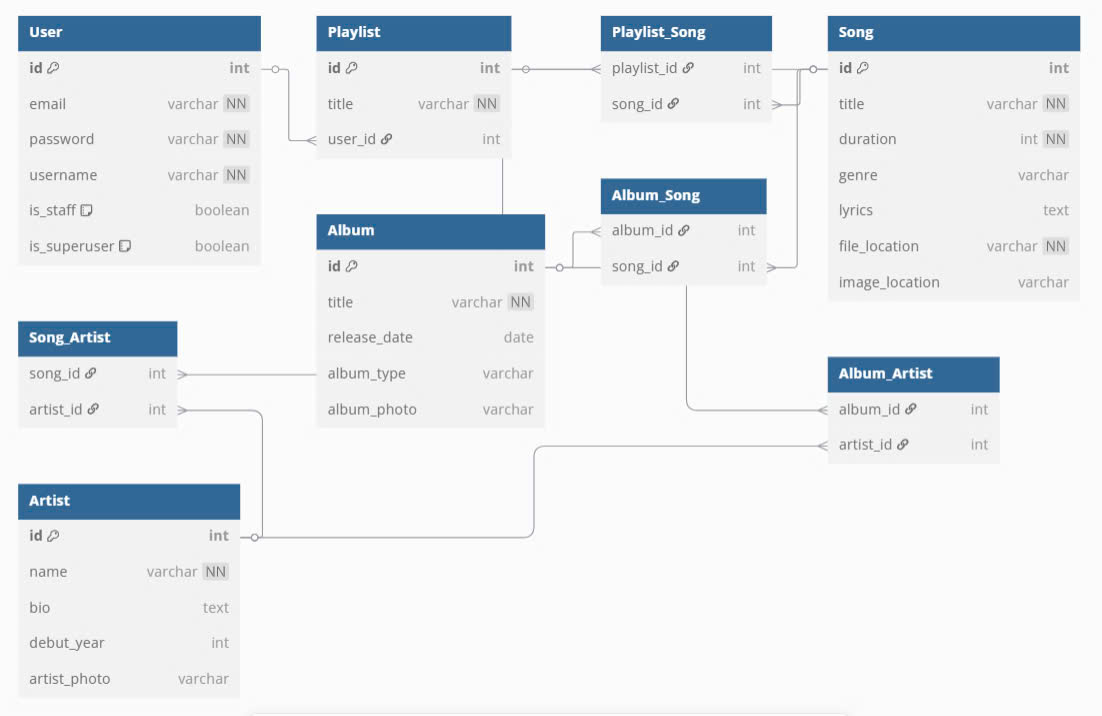
\includegraphics[width=0.8\textwidth]{imgs/erd.png}
    \caption{Sơ đồ ERD của cơ sở dữ liệu}
\end{figure}

\chapter{Hiện thực hệ thống}
\section{Các tính năng chính}
\textbf{API} cung cấp các tính năng chính sau:
\begin{itemize}
    \item \textbf{Đăng ký và đăng nhập người dùng}: 
    \begin{itemize}
        \item Endpoint \texttt{/api/register/}: Cho phép người dùng tạo tài khoản mới với thông tin như email và mật khẩu.
        \item Endpoint \texttt{/api/login/}: Xác thực thông tin người dùng và trả về token để quản lý phiên đăng nhập.
    \end{itemize}
    \item \textbf{Xác thực và phân quyền người dùng}: 
    \begin{itemize}
        \item Đảm bảo chỉ những người dùng được phép mới có thể truy cập các tài nguyên cụ thể thông qua token xác thực.
    \end{itemize}
    \item \textbf{Quản lý thông tin người dùng (CRUD)}: 
    \begin{itemize}
        \item Endpoint \texttt{/api/users/}: Cho phép thêm, sửa, xóa và xem thông tin người dùng.
    \end{itemize}
    \item \textbf{Gửi email xác minh tài khoản}: 
    \begin{itemize}
        \item Endpoint \texttt{/api/verify-email/}: Gửi email xác minh để kích hoạt tài khoản người dùng.
    \end{itemize}
    \item \textbf{Quản lý nhạc và video âm nhạc}:
    \begin{itemize}
        \item Endpoint \texttt{/api/songs/}: Hiển thị danh sách bài hát.
        \item Endpoint \texttt{/api/songs/<id>/}: Hiển thị chi tiết bài hát.
        \item Endpoint \texttt{/api/songs/}: Cho phép thêm bài hát mới (POST).
        \item Endpoint \texttt{/api/songs/<id>/}: Chỉnh sửa bài hát (PUT/PATCH).
        \item Endpoint \texttt{/api/songs/<id>/}: Xóa bài hát (DELETE).
        \item Endpoint \texttt{/api/songs/search/}: Tìm kiếm bài hát theo tên, nghệ sĩ hoặc thể loại.
        \item Endpoint \texttt{/api/videos/}: Quản lý video âm nhạc (tương tự như bài hát).
    \end{itemize}
    \item \textbf{Quản lý danh sách phát và album}:
    \begin{itemize}
        \item Endpoint \texttt{/api/playlists/}: Quản lý danh sách phát nhạc của người dùng.
        \item Endpoint \texttt{/api/albums/}: Cho phép người dùng tạo album nhạc cá nhân.
    \end{itemize}
    \item \textbf{Quản lý yêu thích}:
    \begin{itemize}
        \item Endpoint \texttt{/api/favorites/}: Quản lý danh sách bài hát yêu thích của người dùng.
    \end{itemize}
\end{itemize}

\textbf{Frontend} cung cấp các tính năng chính sau:
\begin{itemize}
    \item \textbf{Giao diện đăng ký và đăng nhập}:
    \begin{itemize}
        \item Người dùng có thể đăng ký tài khoản mới hoặc đăng nhập vào hệ thống thông qua giao diện thân thiện.
    \end{itemize}
    \item \textbf{Giao diện phát nhạc trực tuyến}:
    \begin{itemize}
        \item Tích hợp trình phát nhạc, cho phép người dùng nghe nhạc trực tuyến.
        \item Hỗ trợ phát video âm nhạc.
    \end{itemize}
    \item \textbf{Giao diện quản lý danh sách phát nhạc và album}:
    \begin{itemize}
        \item Người dùng có thể tạo, chỉnh sửa, xóa danh sách phát và album cá nhân.
    \end{itemize}
    \item \textbf{Giao diện quản lý yêu thích}:
    \begin{itemize}
        \item Hiển thị danh sách bài hát yêu thích của người dùng.
    \end{itemize}
    \item \textbf{Trang Admin}:
    \begin{itemize}
        \item Quản trị viên có thể quản lý người dùng, bài hát, video, và thể loại nhạc thông qua giao diện quản trị.
    \end{itemize}
    \item \textbf{Tìm kiếm và khám phá}:
    \begin{itemize}
        \item Người dùng có thể tìm kiếm bài hát, nghệ sĩ, hoặc thể loại nhạc thông qua giao diện tìm kiếm.
    \end{itemize}
    \item \textbf{Tính năng chat (Optional)}:
    \begin{itemize}
        \item Tích hợp tính năng chat trong giao diện web để người dùng có thể tương tác với nhau.
    \end{itemize}
    \begin{figure}[h]
    \centering
    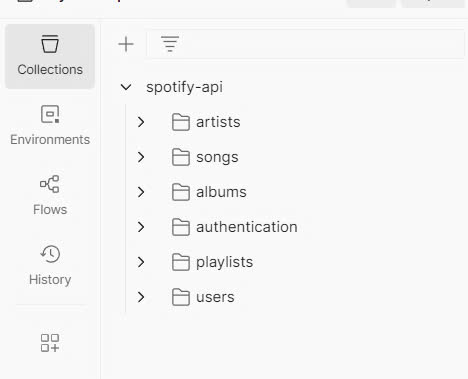
\includegraphics[width=1\textwidth]{imgs/api-postman.jpg}
    \caption{API trên Postman}
\end{figure}
\end{itemize}

\section{Giao diện và hình ảnh minh họa}

\subsection{Quản lý nhạc}

\subsubsection{Hiển thị danh sách}
API cung cấp endpoint \texttt{/api/songs/} để lấy danh sách các bài hát trong hệ thống. Frontend hiển thị danh sách này với các thông tin cơ bản như tên bài hát, nghệ sĩ, và thể loại để người dùng có thể dễ dàng duyệt qua.

\begin{figure}[H]
    \centering
    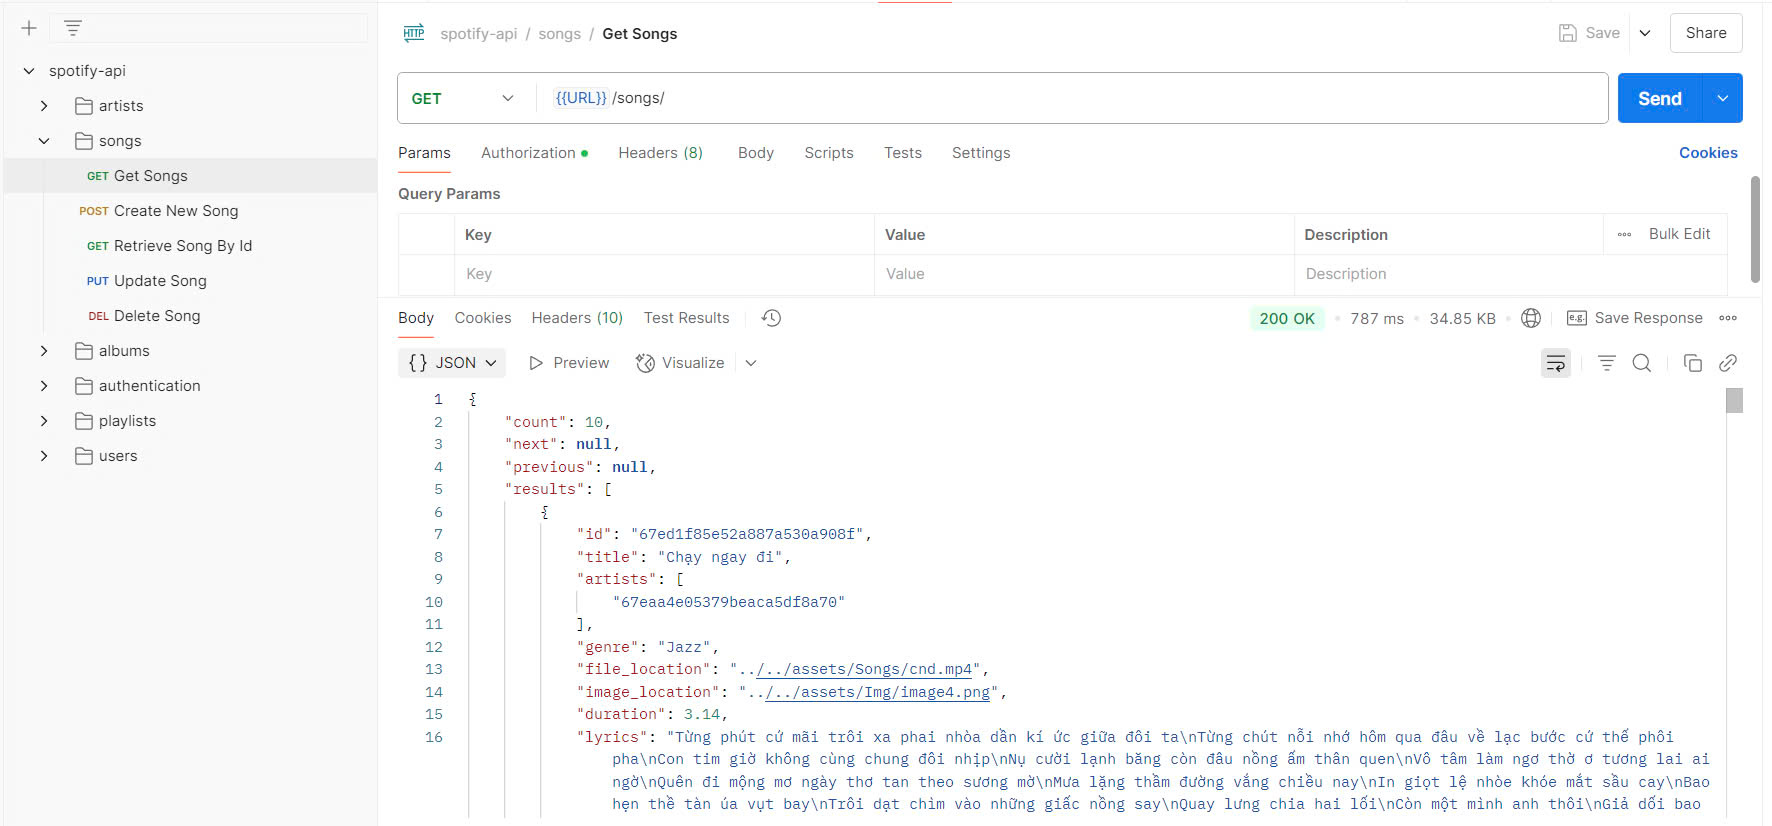
\includegraphics[width=1\textwidth]{imgs/api-songs.jpg}
    \caption{API lấy danh sách bài hát (Postman)}
\end{figure}

\begin{figure}[H]
    \centering
    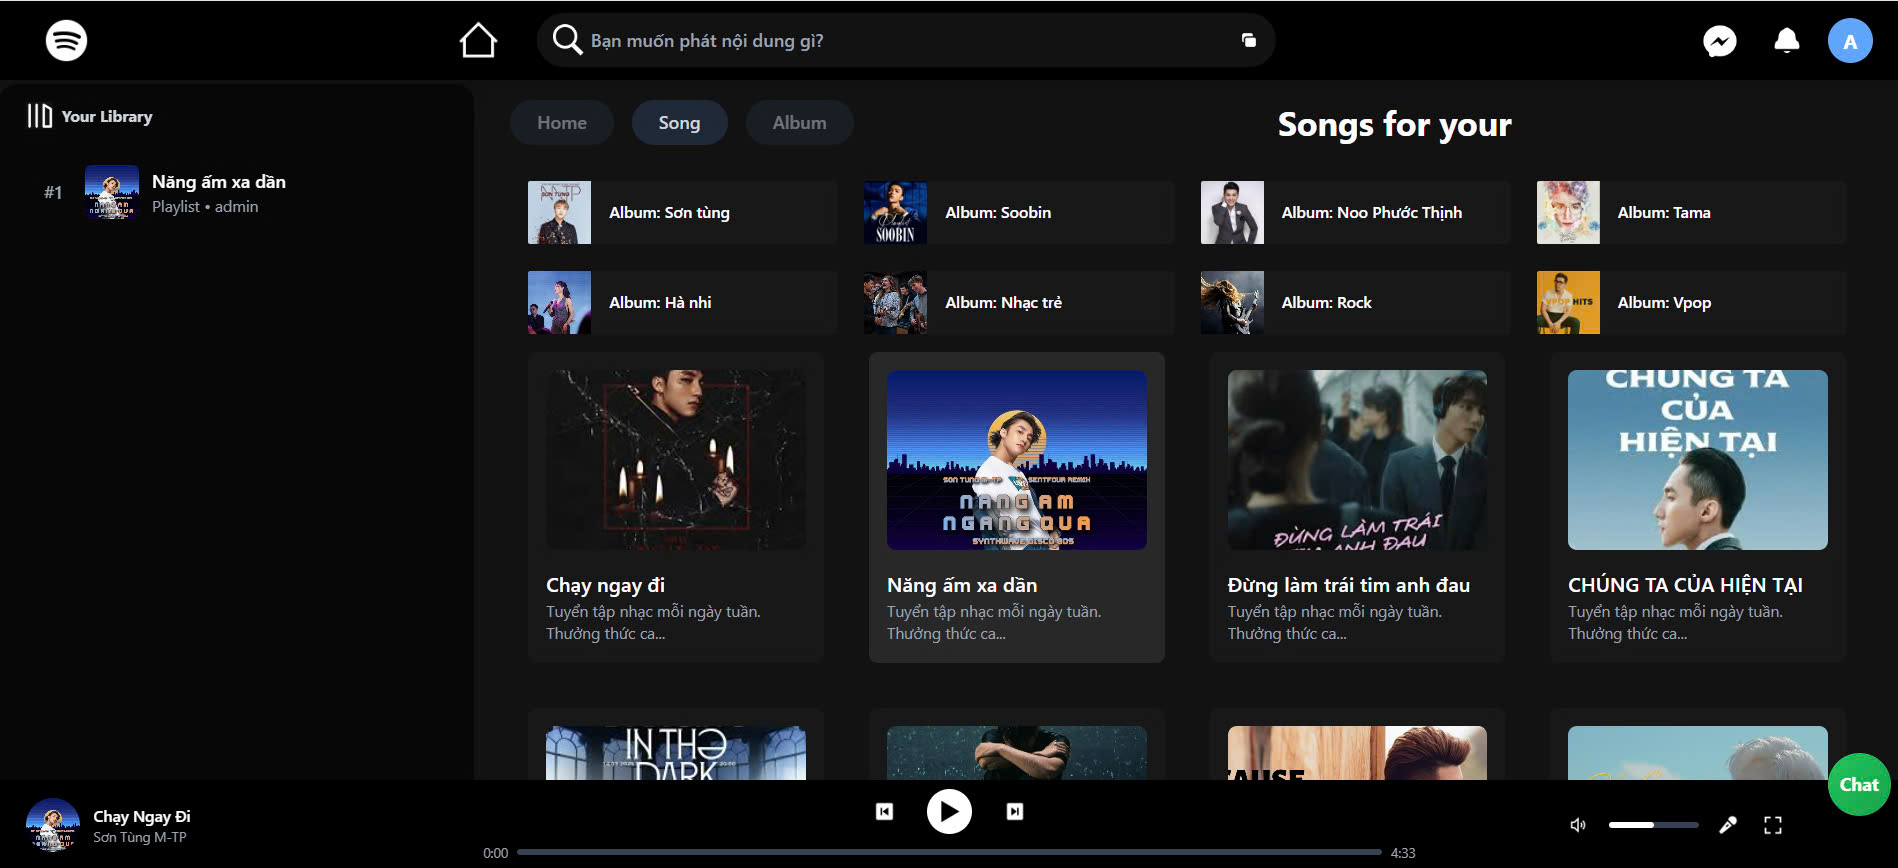
\includegraphics[width=1\textwidth]{imgs/frontend-songs.jpg}
    \caption{Giao diện danh sách bài hát (Frontend)}
\end{figure}
\begin{figure}[H]
    \centering
    \includegraphics[width=1\textwidth]{imgs/frontend-admin-songs.jpg}
    \caption{Giao diện danh sách bài hát trên admin}
\end{figure}

\subsubsection{Hiển thị chi tiết bài hát}
Người dùng có thể xem chi tiết bài hát thông qua endpoint \texttt{/api/songs/<id>/}. Endpoint này trả về các thông tin chi tiết của bài hát như tên bài hát, nghệ sĩ, album, thời gian phát, và lời bài hát.

\begin{figure}[H]
    \centering
    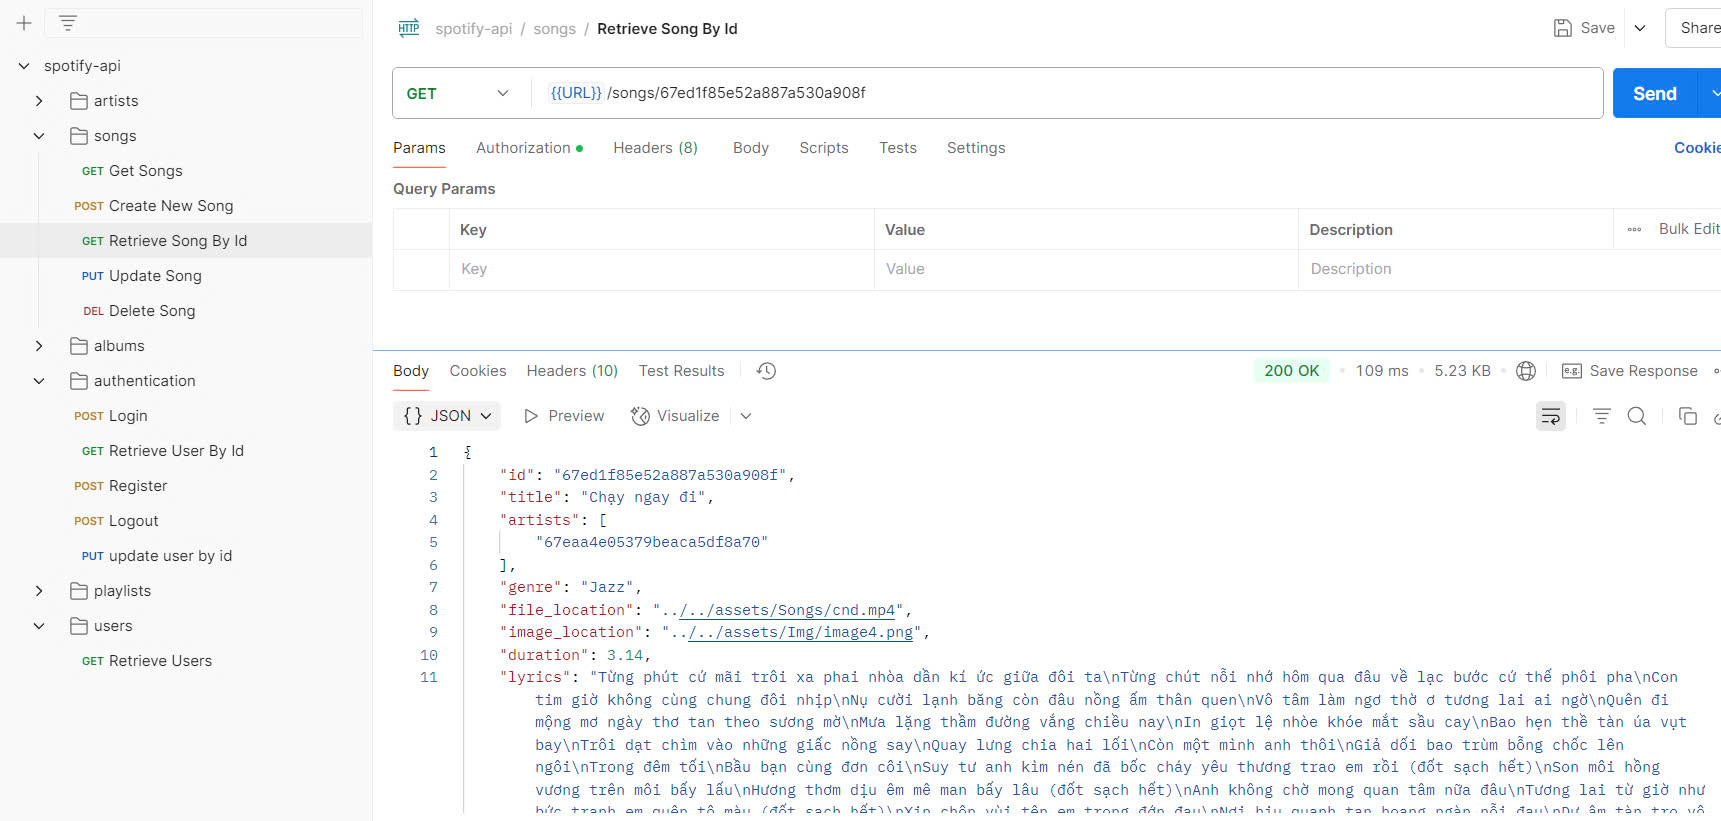
\includegraphics[width=1\textwidth]{imgs/api-song-detail.jpg}
    \caption{API chi tiết bài hát (Postman)}
\end{figure}

\begin{figure}[H]
    \centering
    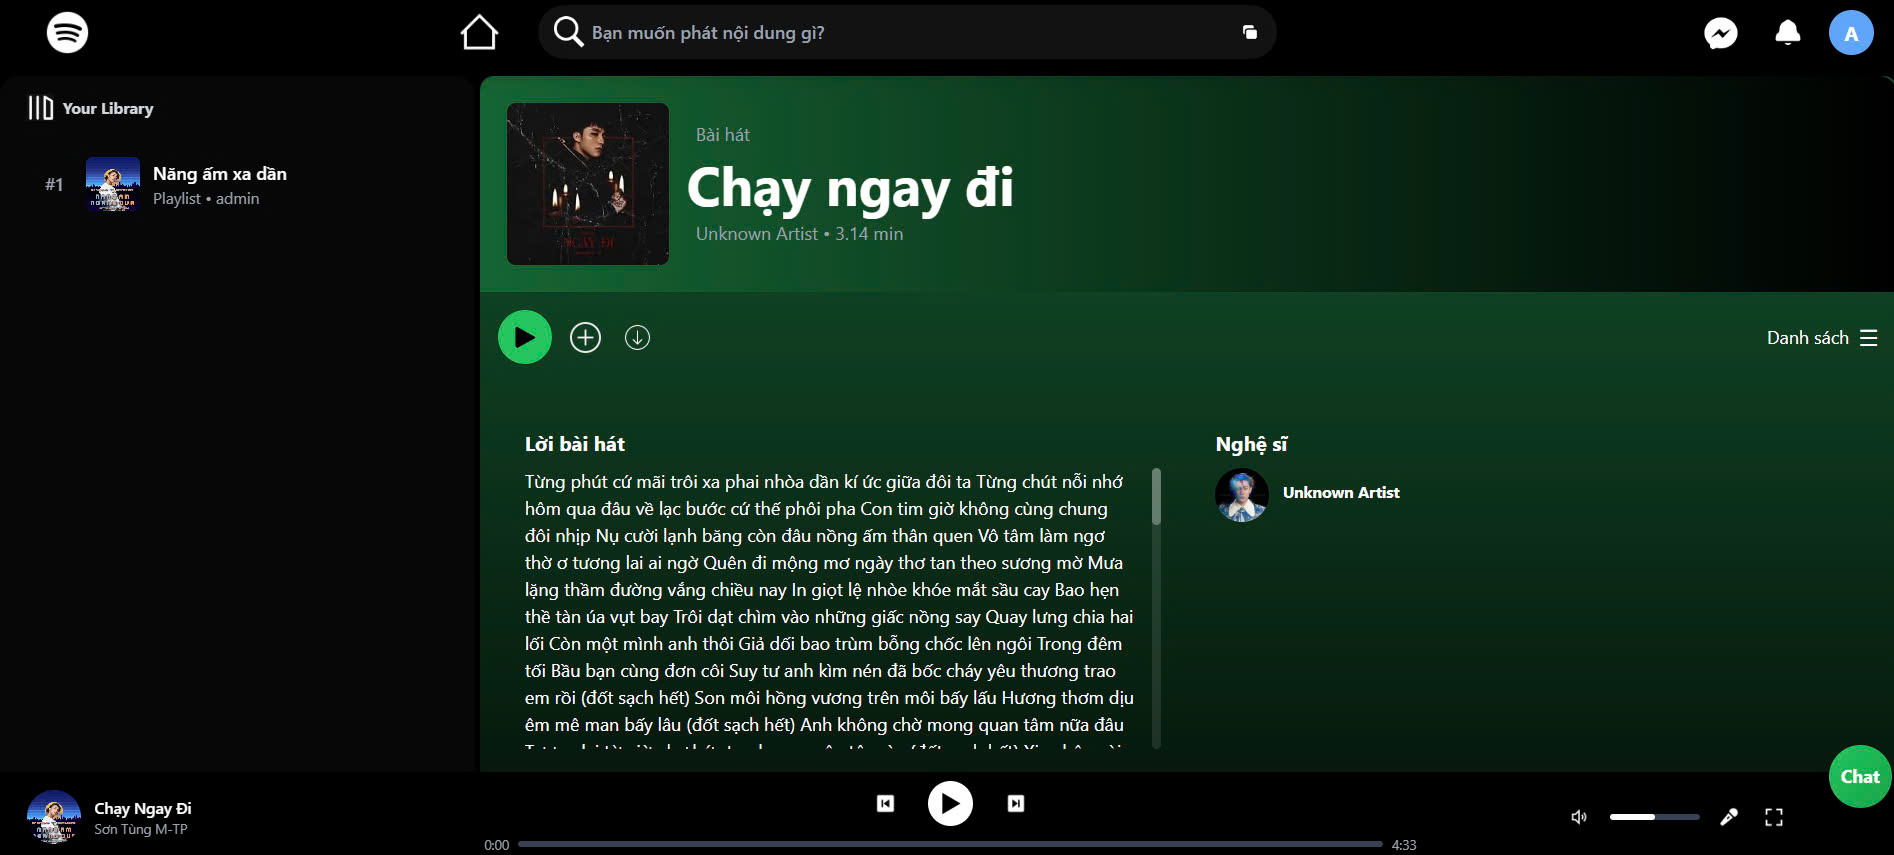
\includegraphics[width=1\textwidth]{imgs/frontend-song-detail.jpg}
    \caption{Giao diện chi tiết bài hát (Frontend)}
\end{figure}

\subsubsection{Nghe thử bài hát}
Frontend tích hợp trình phát nhạc, cho phép người dùng nghe thử bài hát trực tuyến thông qua URL phát nhạc được trả về từ API. Người dùng chỉ cần nhấn vào bài hát để bắt đầu nghe.

\begin{figure}[H]
    \centering
    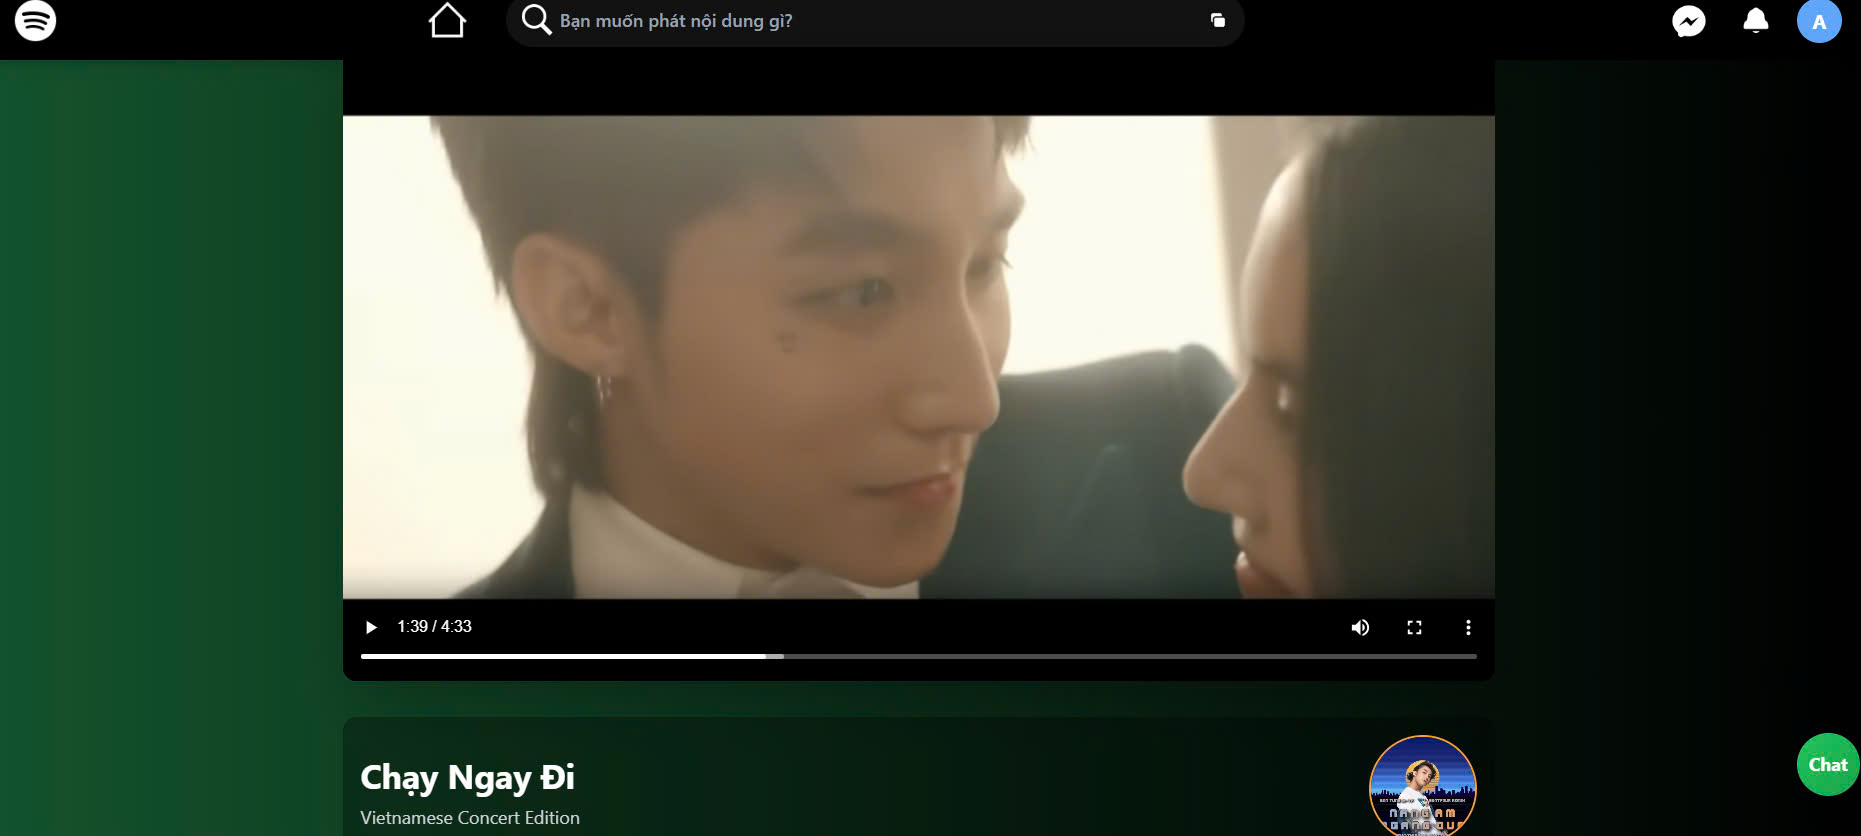
\includegraphics[width=1\textwidth]{imgs/frontend-player.jpg}
    \caption{Giao diện trình phát nhạc}
\end{figure}

\subsubsection{Thêm bài hát mới}
Quản trị viên có thể thêm bài hát mới vào hệ thống thông qua endpoint \texttt{/api/songs/} với phương thức POST. Dữ liệu cần thiết bao gồm tên bài hát, nghệ sĩ, thể loại, URL phát nhạc, và các thông tin liên quan khác.

\begin{figure}[H]
    \centering
    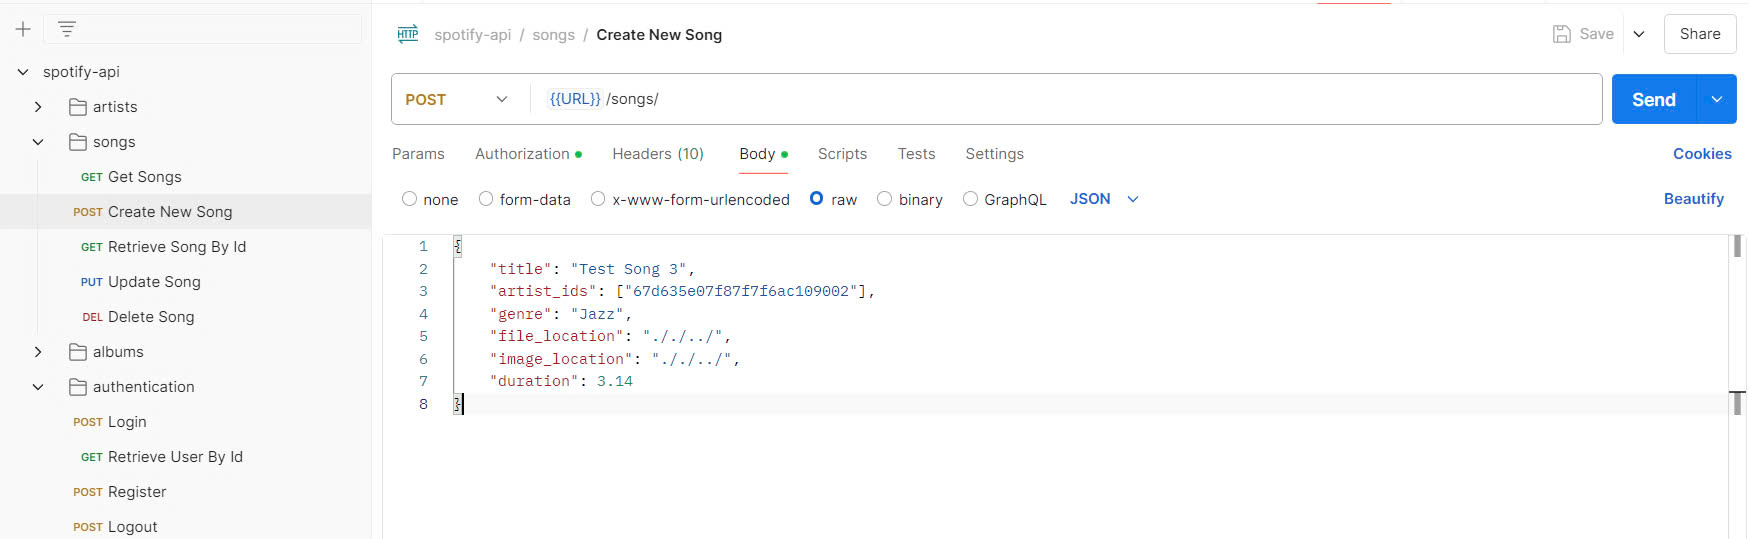
\includegraphics[width=1\textwidth]{imgs/api-add-song.jpg}
    \caption{API thêm bài hát (POST)}
\end{figure}

\begin{figure}[H]
    \centering
    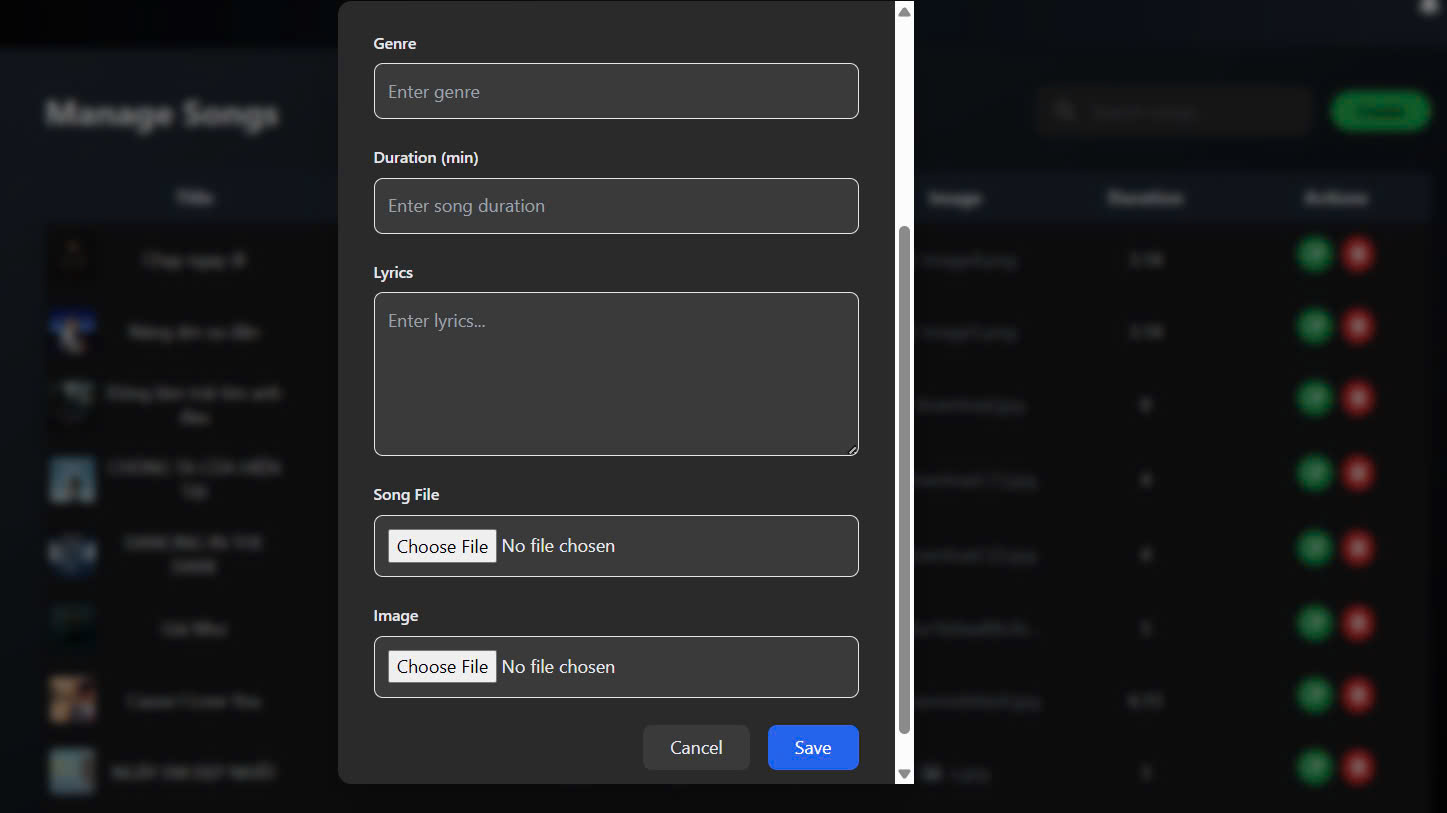
\includegraphics[width=1\textwidth]{imgs/frontend-add-song.jpg}
    \caption{Giao diện thêm bài hát}
\end{figure}

\subsubsection{Chỉnh sửa bài hát}
Quản trị viên có thể chỉnh sửa thông tin bài hát thông qua endpoint \texttt{/api/songs/<id>/} với phương thức PUT hoặc PATCH. Các thông tin có thể chỉnh sửa bao gồm tên bài hát, nghệ sĩ, thể loại, và URL phát nhạc.

\begin{figure}[H]
    \centering
    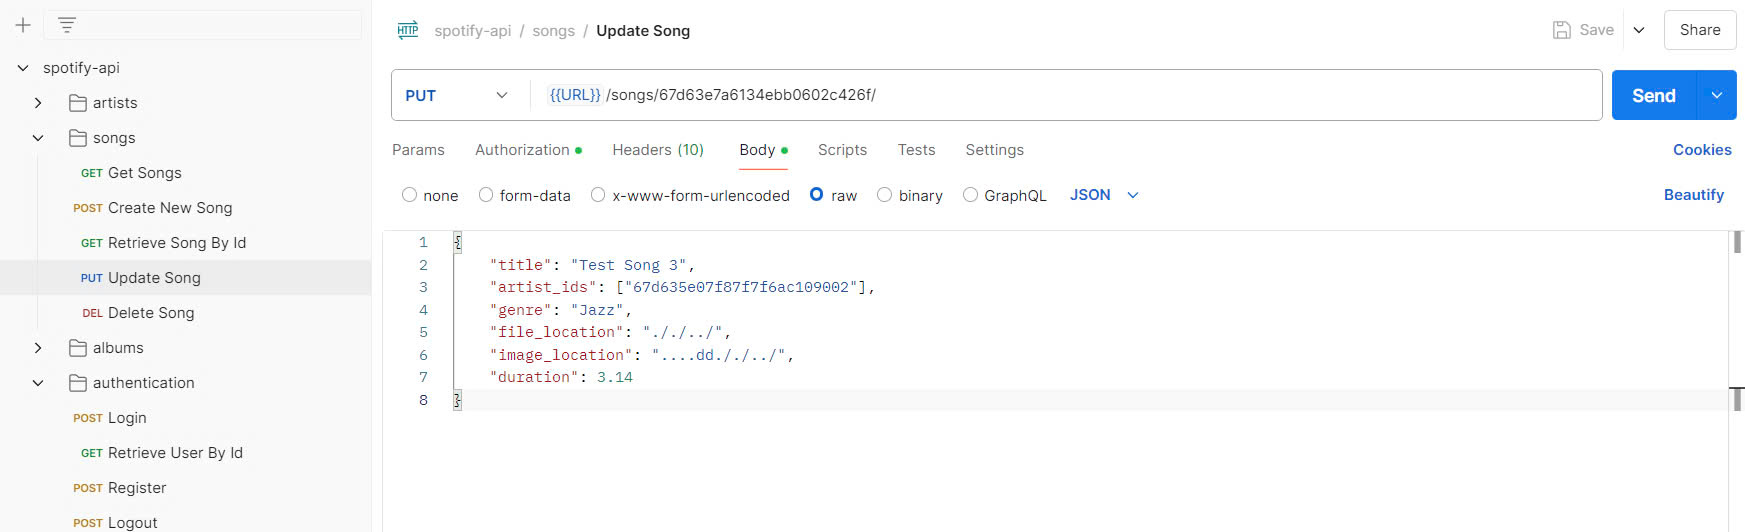
\includegraphics[width=1\textwidth]{imgs/api-edit-song.jpg}
    \caption{API chỉnh sửa bài hát (PUT)}
\end{figure}

\begin{figure}[H]
    \centering
    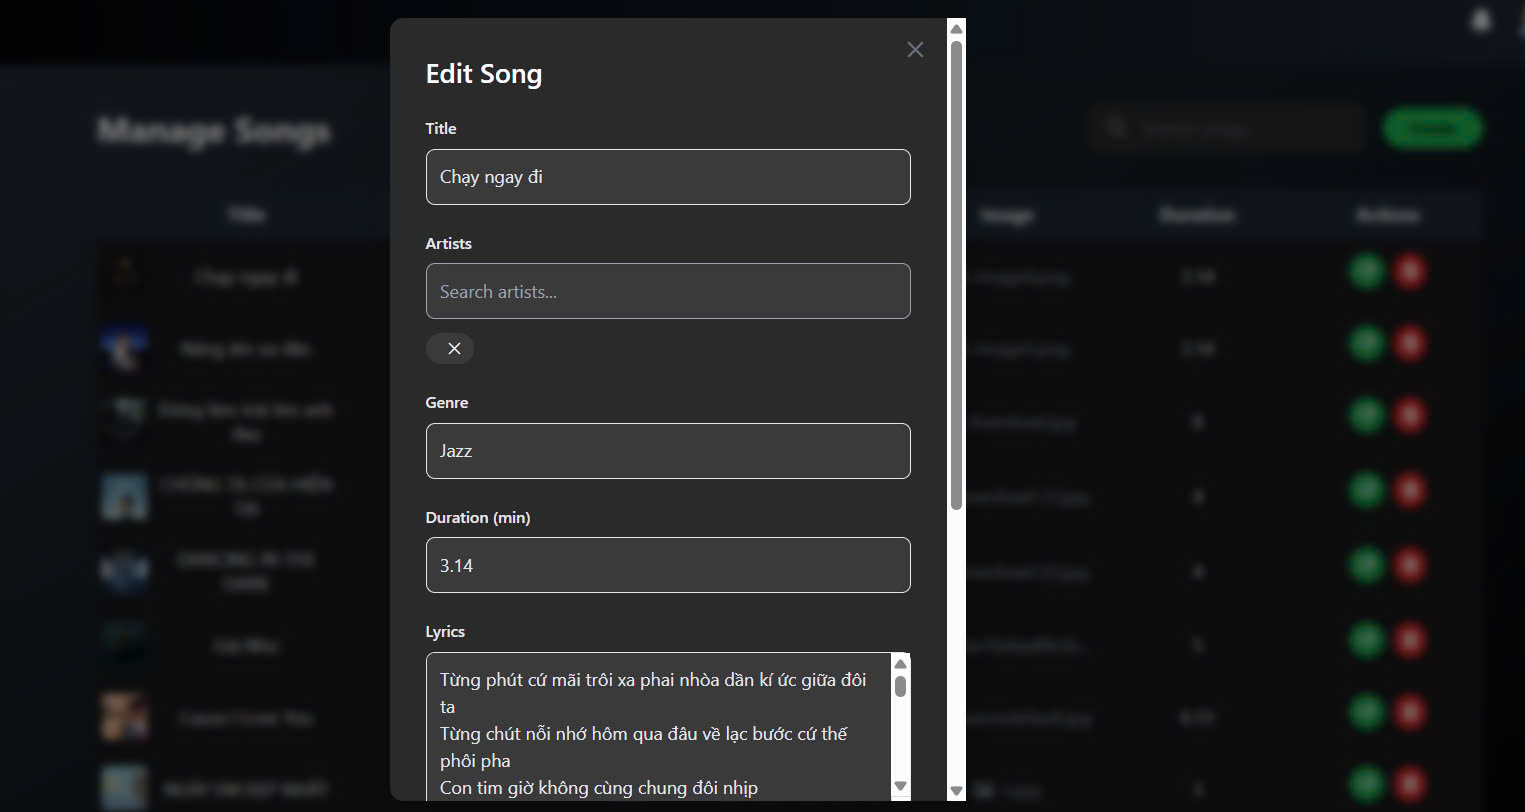
\includegraphics[width=1\textwidth]{imgs/frontend-edit-song.jpg}
    \caption{Giao diện chỉnh sửa bài hát}
\end{figure}

\subsubsection{Xóa nhạc}
Endpoint \texttt{/api/songs/<id>/} với phương thức DELETE cho phép quản trị viên xóa bài hát khỏi hệ thống khi không còn cần thiết. Khi nhấn vào icon delete thì bài hát được xóa và thông báo thành công

\begin{figure}[H]
    \centering
    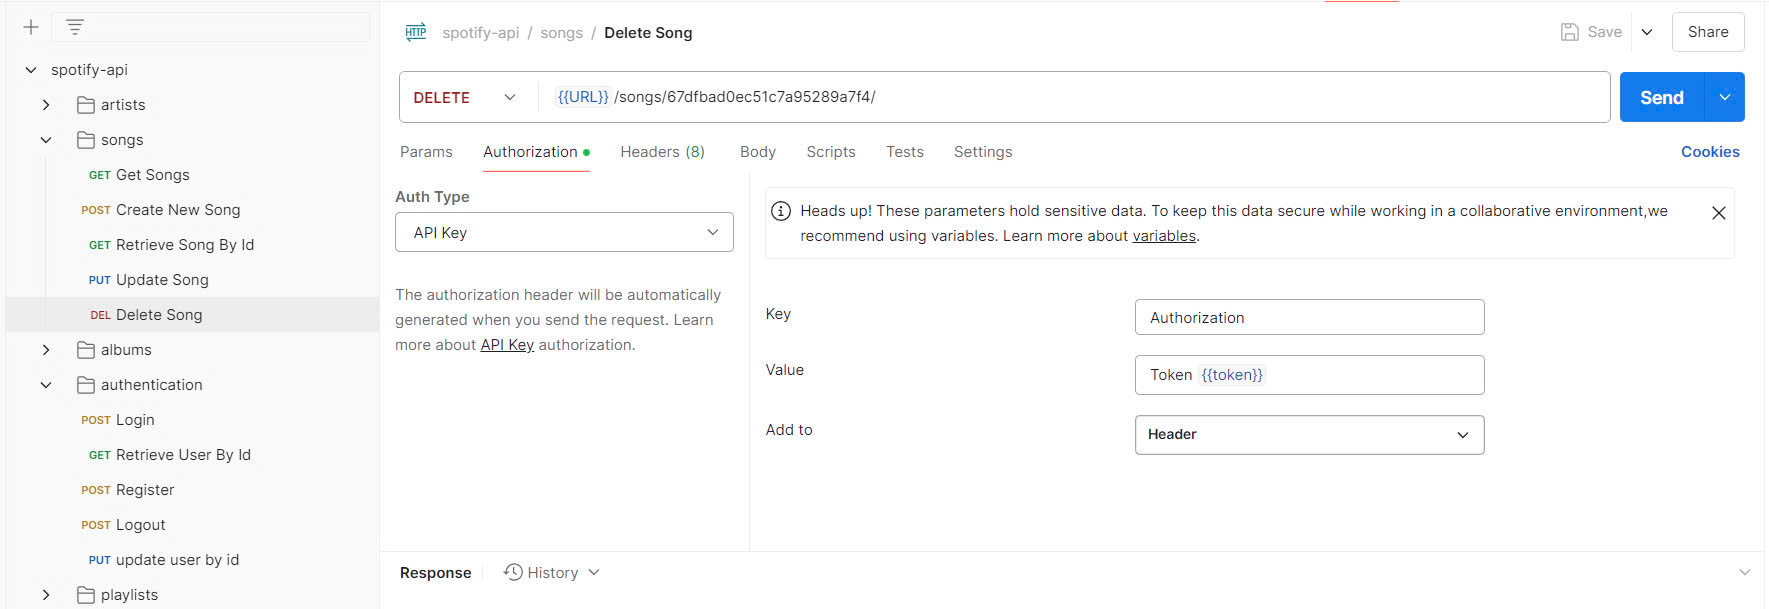
\includegraphics[width=1\textwidth]{imgs/api-delete-song.jpg}
    \caption{API xóa bài hát (DELETE)}
\end{figure}

\begin{figure}[H]
    \centering
    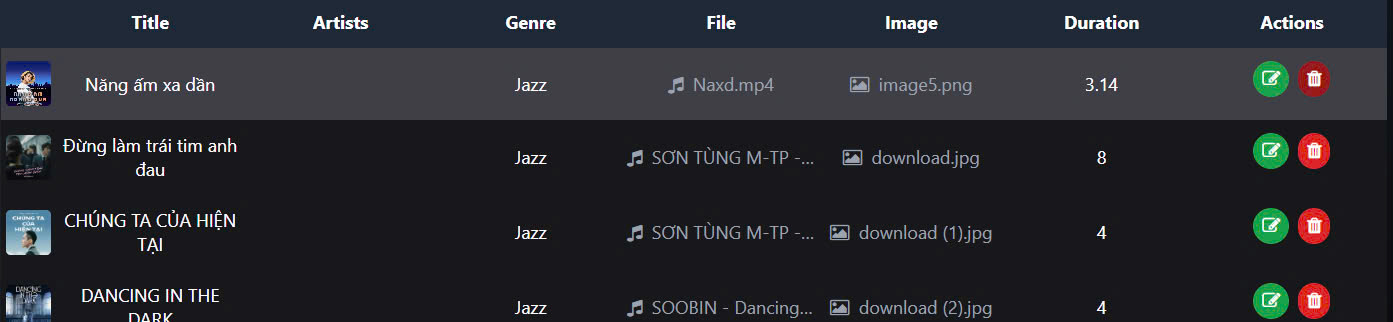
\includegraphics[width=1\textwidth]{imgs/frontend-delete-song.jpg}
    \caption{Giao diện xóa bài hát}
\end{figure}

\subsubsection{Tìm kiếm nhạc}
Hỗ trợ tìm kiếm bài hát qua endpoint, cho phép người dùng tìm kiếm bài hát theo các tiêu chí như tên bài hát, nghệ sĩ, hoặc thể loại.

\begin{figure}[H]
    \centering
    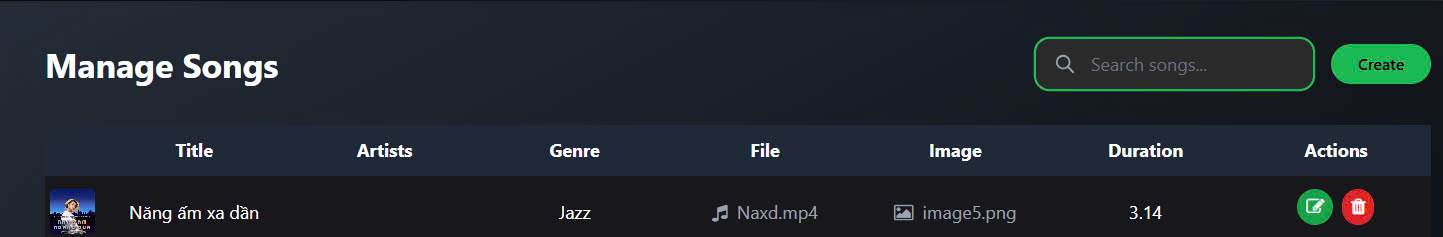
\includegraphics[width=1\textwidth]{imgs/frontend-search-song.jpg}
    \caption{Giao diện tìm kiếm bài hát}
\end{figure}

\section{Quản lý albums}
\subsection{Hiển thị danh sách}
Endpoint \texttt{/api/albums/} trả về danh sách các album có sẵn trong hệ thống. Frontend hiển thị danh sách này với các thông tin như tên album, ngày phát hành, nghệ sĩ liên quan, và ảnh đại diện.

\subsection{Hiển thị chi tiết album}
Người dùng có thể xem chi tiết về một album qua endpoint \texttt{/api/albums/<id>/}, bao gồm thông tin như tên album, ngày phát hành, danh sách bài hát, và nghệ sĩ liên quan.

\subsection{Thêm album}
Quản trị viên có thể thêm album mới vào hệ thống thông qua endpoint \texttt{/api/albums/} với phương thức POST. Dữ liệu cần thiết bao gồm:
\begin{itemize}
    \item \textbf{title}: Tên album.
    \item \textbf{release\_date}: Ngày phát hành.
    \item \textbf{album\_type}: Loại album (ví dụ: single, album đầy đủ).
    \item \textbf{artist\_ids}: Danh sách ID nghệ sĩ liên quan.
    \item \textbf{song\_ids}: Danh sách ID bài hát trong album.
    \item \textbf{image\_file}: Ảnh đại diện của album.
\end{itemize}

\subsection{Chỉnh sửa album}
Endpoint \texttt{/api/albums/<id>/} với phương thức PUT hoặc PATCH cho phép chỉnh sửa thông tin album, bao gồm tên, ngày phát hành, danh sách bài hát, và nghệ sĩ liên quan.

\subsection{Xóa album}
Quản trị viên có thể xóa album khỏi hệ thống qua endpoint \texttt{/api/albums/<id>/} với phương thức DELETE.

\section{Quản lý nghệ sĩ (artists)}
\subsection{Hiển thị danh sách}
Endpoint \texttt{/api/artists/} trả về danh sách các nghệ sĩ trong hệ thống. Frontend hiển thị danh sách này với các thông tin như tên nghệ sĩ, năm ra mắt, và ảnh đại diện.

\subsection{Hiển thị chi tiết nghệ sĩ}
Người dùng có thể xem chi tiết về một nghệ sĩ qua endpoint \texttt{/api/artists/<id>/}, bao gồm thông tin như tên, tiểu sử, năm ra mắt, và danh sách album hoặc bài hát liên quan.

\subsection{Thêm nghệ sĩ}
Quản trị viên có thể thêm nghệ sĩ mới vào hệ thống thông qua endpoint \texttt{/api/artists/} với phương thức POST. Dữ liệu cần thiết bao gồm:
\begin{itemize}
    \item \textbf{name}: Tên nghệ sĩ.
    \item \textbf{bio}: Tiểu sử.
    \item \textbf{debut\_year}: Năm ra mắt.
    \item \textbf{artist\_photo}: Ảnh đại diện của nghệ sĩ.
\end{itemize}

\subsection{Chỉnh sửa nghệ sĩ}
Endpoint \texttt{/api/artists/<id>/} với phương thức PUT hoặc PATCH cho phép chỉnh sửa thông tin nghệ sĩ, bao gồm tên, tiểu sử, năm ra mắt, và ảnh đại diện.

\subsection{Xóa nghệ sĩ}
Quản trị viên có thể xóa nghệ sĩ khỏi hệ thống qua endpoint \texttt{/api/artists/<id>/} với phương thức DELETE.

\section{Quản lý người dùng (users)}
\subsection{Hiển thị danh sách}
Endpoint \texttt{/api/users/} trả về danh sách tất cả người dùng trong hệ thống. Quản trị viên có thể sử dụng endpoint này để theo dõi và quản lý người dùng. Frontend hiển thị danh sách với các thông tin như tên người dùng, email, vai trò, và trạng thái tài khoản.

\subsection{Hiển thị chi tiết người dùng}
Quản trị viên có thể xem chi tiết thông tin của một người dùng qua endpoint \texttt{/api/users/<id>/}, bao gồm các thông tin như tên người dùng, email, vai trò, và các thông tin cá nhân khác.

\subsection{Thêm người dùng}
Quản trị viên có thể thêm người dùng mới vào hệ thống thông qua endpoint \texttt{/api/users/} với phương thức POST. Dữ liệu cần thiết bao gồm:
\begin{itemize}
    \item \textbf{username}: Tên đăng nhập.
    \item \textbf{email}: Địa chỉ email.
    \item \textbf{password}: Mật khẩu.
    \item \textbf{isstaff}: Vai trò (admin hoặc user).
     \item \textbf{issuperuser}: Quyền....
\end{itemize}

\subsection{Chỉnh sửa người dùng}
Endpoint \texttt{/api/users/<id>/} với phương thức PUT hoặc PATCH cho phép chỉnh sửa thông tin người dùng, bao gồm tên, email, và vai trò.

\subsection{Xóa người dùng}
Quản trị viên có thể xóa người dùng khỏi hệ thống qua endpoint \texttt{/api/users/<id>/} với phương thức DELETE.

\section{Quản lý server}
\subsection{Khởi động server}
Server có thể được khởi động bằng lệnh \texttt{python manage.py runserver}, sau khi môi trường đã được cấu hình và ứng dụng đã được cài đặt đầy đủ.

\subsection{Tắt server}
Để tắt server, người dùng chỉ cần dừng tiến trình đang chạy trong terminal bằng cách sử dụng lệnh \texttt{CTRL+C} hoặc tắt ứng dụng trực tiếp từ quản lý dịch vụ.

\section{Frontend Client}
\subsection{Đăng nhập}
Người dùng có thể đăng nhập vào hệ thống thông qua giao diện frontend. Thông tin đăng nhập sẽ được gửi đến endpoint \texttt{/api/login/} để xác thực và nhận token cho các yêu cầu tiếp theo.

\subsection{Đăng ký}
Người dùng có thể đăng ký tài khoản mới qua giao diện frontend. Các thông tin đăng ký được gửi đến endpoint \texttt{/api/register/} để tạo tài khoản mới trong hệ thống.

\subsection{Trang chủ}
Trang chủ hiển thị danh sách các bài hát nổi bật, danh sách phát được đề xuất và các thể loại nhạc phổ biến. Người dùng có thể duyệt qua và chọn bài hát yêu thích.

\subsection{Tìm kiếm}
Người dùng có thể tìm kiếm bài hát, nghệ sĩ hoặc thể loại qua giao diện tìm kiếm. Thông tin tìm kiếm sẽ được gửi đến endpoint \texttt{/api/songs/search/} để trả về kết quả phù hợp.

\subsection{Nghe nhạc}
Frontend tích hợp trình phát nhạc, cho phép người dùng phát bài hát trực tiếp từ URL phát nhạc được trả về từ API. Người dùng có thể nghe bài hát mà không cần rời khỏi giao diện.

\subsection{PlayList}
Người dùng có thể tạo, chỉnh sửa và xóa danh sách phát cá nhân. API cung cấp các endpoint như \texttt{/api/playlists/} để quản lý danh sách phát của người dùng.
\subsection{User tạo album}
Người dùng có thể thêm .....
\subsection{Danh sách yêu thích}
Người dùng có thể thêm bài hát vào danh sách yêu thích của mình. API cung cấp endpoint \texttt{/api/favorites/} để quản lý danh sách bài hát yêu thích này.

\subsection{Tài khoản cá nhân}
Người dùng có thể xem và chỉnh sửa thông tin tài khoản cá nhân của mình qua giao diện frontend. Thông tin thay đổi sẽ được gửi đến endpoint \texttt{/api/users/<id>/} để cập nhật trong hệ thống.

\documentclass[12pt,a4paper]{article}
\usepackage[utf8]{vietnam}
\usepackage{graphicx}
\usepackage{hyperref}
\usepackage{listings}
\usepackage{xcolor}
\usepackage{tcolorbox}
\usepackage{geometry}
\usepackage{fancyhdr}
\usepackage{titlesec}

\geometry{a4paper, margin=2.5cm}

\hypersetup{
    colorlinks=true,
    linkcolor=blue,
    filecolor=magenta,
    urlcolor=blue,
}

\lstset{
    backgroundcolor=\color{gray!10},
    basicstyle=\ttfamily\small,
    breaklines=true,
    captionpos=b,
    commentstyle=\color{green!50!black},
    keywordstyle=\color{blue},
    stringstyle=\color{red},
    numberstyle=\tiny\color{gray},
    numbers=left,
    numbersep=5pt,
    frame=single,
    framesep=5pt,
    rulecolor=\color{black!30},
    tabsize=4
}

% Định dạng heading cho section
\titleformat{\section}
  {\LARGE\bfseries\centering}
  {}
  {0em}
  {}
  []

% Bỏ title và author
\date{}

\begin{document}

\begin{center}
    \Huge\textbf{BÁO CÁO DỰ ÁN}
\end{center}

\section*{I. BACKEND}

% Nội dung từ đoạn code Backend
\section{Cài đặt Python}

Python là ngôn ngữ lập trình cốt lõi cho dự án Django của chúng ta. Django 5.0.13 yêu cầu Python phiên bản 3.10 trở lên.

\subsection{Bước 1: Tải và cài đặt Python}

\begin{enumerate}
    \item Truy cập trang web chính thức của Python tại \url{https://www.python.org/downloads/}
    \item Tải phiên bản Python phù hợp (khuyến nghị Python 3.10 hoặc cao hơn)
    \item Trong quá trình cài đặt, đảm bảo tích vào tùy chọn "Add Python to PATH"
\end{enumerate}

\begin{tcolorbox}[colback=yellow!10, colframe=yellow!50!black, title=Lưu ý quan trọng]
Đối với người dùng Windows, việc thêm Python vào biến môi trường PATH là rất quan trọng để có thể chạy Python từ Command Prompt hoặc PowerShell.
\end{tcolorbox}

\subsection{Bước 2: Xác nhận cài đặt thành công}

Mở Command Prompt (Windows) hoặc Terminal (macOS/Linux) và chạy lệnh:

\begin{lstlisting}[language=bash]
python --version
\end{lstlisting}

hoặc

\begin{lstlisting}[language=bash]
python3 --version
\end{lstlisting}

\begin{figure}[h]
    \centering
    \includegraphics[width=0.7\linewidth]{python_version.png}
    \caption{Kết quả lệnh kiểm tra phiên bản Python}
    \label{fig:python-version}
\end{figure}

\section{Cài đặt MongoDB}

MongoDB là cơ sở dữ liệu NoSQL được sử dụng trong dự án của chúng ta để lưu trữ dữ liệu.

\subsection{Bước 1: Tải và cài đặt MongoDB}

\begin{enumerate}
    \item Truy cập trang web chính thức của MongoDB: \url{https://www.mongodb.com/try/download/community}
    \item Tải phiên bản MongoDB Community Edition phù hợp với hệ điều hành của bạn
    \item Tiến hành cài đặt theo hướng dẫn của trình cài đặt
    \item Đối với Windows, chọn "Complete" trong quá trình cài đặt để cài đặt MongoDB Compass (giao diện đồ họa)
\end{enumerate}

\subsection{Bước 2: Khởi động MongoDB}

\subsubsection{Windows}
MongoDB thường được cài đặt như một dịch vụ và tự khởi động. Nếu không, bạn có thể khởi động thủ công:

\begin{lstlisting}[language=bash]
"C:\Program Files\MongoDB\Server\6.0\bin\mongod.exe" --dbpath="C:\data\db"
\end{lstlisting}

\subsubsection{macOS/Linux}
Mở Terminal và chạy:

\begin{lstlisting}[language=bash]
sudo systemctl start mongod
\end{lstlisting}

\subsection{Bước 3: Kiểm tra kết nối}

Mở terminal hoặc command prompt và chạy:

\begin{lstlisting}[language=bash]
mongosh
\end{lstlisting}

\begin{figure}[h]
    \centering
    \includegraphics[width=0.8\linewidth]{mongodb_running.png}
    \caption{Màn hình MongoDB đang chạy}
    \label{fig:mongodb-running}
\end{figure}

\section{Thiết lập môi trường ảo Python}

Môi trường ảo Python giúp quản lý các phụ thuộc của dự án một cách độc lập, tránh xung đột với các dự án khác.

\subsection{Bước 1: Tạo môi trường ảo}

\begin{lstlisting}[language=bash]
python -m venv myenv
\end{lstlisting}

Lệnh này sẽ tạo một thư mục mới có tên "myenv" chứa môi trường ảo Python.

\subsection{Bước 2: Kích hoạt môi trường ảo}

\subsubsection{Windows}
\begin{lstlisting}[language=bash]
myenv\Scripts\activate
\end{lstlisting}

\subsubsection{macOS/Linux}
\begin{lstlisting}[language=bash]
source myenv/bin/activate
\end{lstlisting}

Khi môi trường ảo được kích hoạt, tên môi trường sẽ xuất hiện trong dấu ngoặc đơn ở đầu dòng lệnh, ví dụ: \texttt{(myenv) C:\Users\username>}

\begin{tcolorbox}[colback=blue!5, colframe=blue!40!black, title=Mẹo]
Để thoát khỏi môi trường ảo, chỉ cần gõ lệnh \texttt{deactivate} trong terminal.
\end{tcolorbox}

\section{Cài đặt các gói phụ thuộc}

\subsection{Bước 1: Tạo file requirements.txt}

Tạo một file văn bản có tên \texttt{requirements.txt} với nội dung sau:

\begin{lstlisting}
asgiref==3.8.1
attrs==25.3.0
autobahn==24.4.2
Automat==25.4.16
boto3==1.37.37
botocore==1.37.37
cffi==1.17.1
channels==4.0.0
constantly==23.10.4
cryptography==44.0.2
daphne==4.0.0
Django==5.0.13
django-cors-headers==4.7.0
django-environ==0.12.0
django-rest-framework-mongoengine==3.4.1
djangorestframework==3.15.2
dnspython==2.7.0
hyperlink==21.0.0
idna==3.10
incremental==24.7.2
jmespath==1.0.1
mongoengine==0.29.1
pyasn1==0.6.1
pyasn1_modules==0.4.2
pycparser==2.22
pymongo==4.11.2
pyOpenSSL==25.0.0
python-dateutil==2.9.0.post0
s3transfer==0.11.5
service-identity==24.2.0
setupt
ools==78.1.1
six==1.17.0
sqlparse==0.5.3
Twisted==24.11.0
txaio==23.1.1
typing_extensions==4.13.2
urllib3==2.4.0
zope.interface==7.2
\end{lstlisting}

\subsection{Bước 2: Cài đặt các gói}

Trong môi trường ảo đã kích hoạt, chạy lệnh sau để cài đặt tất cả các gói phụ thuộc:

\begin{lstlisting}[language=bash]
pip install -r requirements.txt
\end{lstlisting}

\begin{figure}[h]
    \centering
    \includegraphics[width=0.8\linewidth]{pip_install.png}
    \caption{Quá trình cài đặt các gói từ requirements.txt}
    \label{fig:pip-install}
\end{figure}

\subsection{Bước 3: Xác minh cài đặt}

Kiểm tra xem các gói đã được cài đặt thành công bằng lệnh:

\begin{lstlisting}[language=bash]
pip list
\end{lstlisting}

\section{Khởi tạo dự án Django}

\subsection{Bước 1: Tạo dự án mới}

\begin{lstlisting}[language=bash]
django-admin startproject myproject
cd myproject
\end{lstlisting}

\subsection{Bước 2: Cấu hình cơ sở dữ liệu MongoDB}

Mở file \texttt{settings.py} trong thư mục \texttt{myproject} và thêm đoạn mã sau:

\begin{lstlisting}[language=python]
# MongoDB settings
import mongoengine

mongoengine.connect(
    db='myproject',
    host='localhost',
    port=27017
)

# Thêm các ứng dụng vào INSTALLED_APPS
INSTALLED_APPS = [
    'django.contrib.admin',
    'django.contrib.auth',
    'django.contrib.contenttypes',
    'django.contrib.sessions',
    'django.contrib.messages',
    'django.contrib.staticfiles',
    'channels',  # WebSockets
    'rest_framework',  # REST API
    'corsheaders',  # CORS support
]

# Cấu hình Channels
ASGI_APPLICATION = 'myproject.asgi.application'
CHANNEL_LAYERS = {
    'default': {
        'BACKEND': 'channels.layers.InMemoryChannelLayer',
    },
}

# Cấu hình CORS
MIDDLEWARE = [
    'corsheaders.middleware.CorsMiddleware',
    # ... các middleware khác
]

CORS_ALLOW_ALL_ORIGINS = True  # Chỉ dùng cho development

# Cấu hình Twisted
TWISTED_SETTINGS = {
    'reactor': 'twisted.internet.asyncioreactor.AsyncioSelectorReactor',
}
\end{lstlisting}

\subsection{Bước 3: Tạo ứng dụng API}

\begin{lstlisting}[language=bash]
python manage.py startapp api
\end{lstlisting}

\subsection{Bước 4: Cấu hình mô hình MongoDB và serializer}

Tạo file \texttt{models.py} trong thư mục \texttt{api}:

\begin{lstlisting}[language=python]
from mongoengine import Document, StringField, DateTimeField
import datetime

class Item(Document):
    name = StringField(max_length=200, required=True)
    description = StringField()
    created_at = DateTimeField(default=datetime.datetime.now)
\end{lstlisting}

Tạo file \texttt{serializers.py} trong thư mục \texttt{api}:

\begin{lstlisting}[language=python]
from rest_framework_mongoengine import serializers
from .models import Item

class ItemSerializer(serializers.DocumentSerializer):
    class Meta:
        model = Item
        fields = '__all__'
\end{lstlisting}

\subsection{Bước 5: Cấu hình WebSocket Consumer}

Tạo file \texttt{consumers.py} trong thư mục \texttt{api}:

\begin{lstlisting}[language=python]
from channels.generic.websocket import AsyncWebsocketConsumer
import json

class ChatConsumer(AsyncWebsocketConsumer):
    async def connect(self):
        await self.accept()

    async def disconnect(self, close_code):
        pass

    async def receive(self, text_data):
        text_data_json = json.loads(text_data)
        message = text_data_json['message']
        
        await self.send(text_data=json.dumps({
            'message': message
        }))
\end{lstlisting}

\section{Kiểm tra cài đặt}

\subsection{Bước 1: Chạy server phát triển}

\begin{lstlisting}[language=bash]
python manage.py runserver
\end{lstlisting}

\begin{figure}[h]
    \centering
    \includegraphics[width=0.8\linewidth]{django_running.png}
    \caption{Server Django đang chạy thành công}
    \label{fig:django-running}
\end{figure}

\subsection{Bước 2: Kiểm tra kết nối}

Mở trình duyệt web và truy cập địa chỉ: \url{http://127.0.0.1:8000/}

\begin{figure}[h]
    \centering
    \includegraphics[width=0.8\linewidth]{django_welcome.png}
    \caption{Giao diện trang web Django mặc định}
    \label{fig:django-welcome}
\end{figure}

\begin{figure}[h]
    \centering
    \includegraphics[width=0.7\linewidth]{project_structure.png}
    \caption{Cấu trúc thư mục dự án}
    \label{fig:project-structure}
\end{figure}

\section{Cấu hình AWS}

\subsection{Bước 1: Thiết lập credentials AWS}

Để tương tác với các dịch vụ AWS, cần phải có thông tin xác thực AWS. Tạo file credentials tại vị trí thích hợp:

\subsubsection{Windows}
Tạo file tại: \texttt{C:\textbackslash Users\textbackslash YOUR\_USERNAME\textbackslash .aws\textbackslash credentials}

\subsubsection{macOS/Linux}
Tạo file tại: \texttt{\~{}/.aws/credentials}

Nội dung file:

\begin{lstlisting}
[default]
aws_access_key_id = YOUR_ACCESS_KEY
aws_secret_access_key = YOUR_SECRET_KEY
\end{lstlisting}

\subsection{Bước 2: Cấu hình AWS trong Django}

Thêm đoạn mã sau vào file \texttt{settings.py}:

\begin{lstlisting}[language=python]
# AWS S3 Configuration
AWS_ACCESS_KEY_ID = 'YOUR_ACCESS_KEY'
AWS_SECRET_ACCESS_KEY = 'YOUR_SECRET_KEY'
AWS_STORAGE_BUCKET_NAME = 'your-bucket-name'
AWS_S3_REGION_NAME = 'your-region'
DEFAULT_FILE_STORAGE = 'storages.backends.s3boto3.S3Boto3Storage'
\end{lstlisting}

\begin{tcolorbox}[colback=red!5, colframe=red!50!black, title=Cảnh báo bảo mật]
Không bao giờ lưu trữ khóa AWS hoặc bất kỳ thông tin xác thực nào trực tiếp trong mã nguồn hoặc đưa lên hệ thống kiểm soát phiên bản như GitHub. Thay vào đó, sử dụng biến môi trường hoặc file .env kết hợp với django-environ.
\end{tcolorbox}

\subsection{Bước 3: Sử dụng biến môi trường an toàn}

Tạo file \texttt{.env} trong thư mục gốc của dự án:

\begin{lstlisting}
AWS_ACCESS_KEY_ID=your_access_key
AWS_SECRET_ACCESS_KEY=your_secret_key
AWS_STORAGE_BUCKET_NAME=your_bucket
AWS_S3_REGION_NAME=your_region
\end{lstlisting}

Và cập nhật \texttt{settings.py} để sử dụng django-environ:

\begin{lstlisting}[language=python]
import environ

env = environ.Env()
environ.Env.read_env()  # Đọc file .env

# AWS S3 Configuration
AWS_ACCESS_KEY_ID = env('AWS_ACCESS_KEY_ID')
AWS_SECRET_ACCESS_KEY = env('AWS_SECRET_ACCESS_KEY')
AWS_STORAGE_BUCKET_NAME = env('AWS_STORAGE_BUCKET_NAME')
AWS_S3_REGION_NAME = env('AWS_S3_REGION_NAME')
\end{lstlisting}

\section{Kết luận}

Báo cáo này đã hướng dẫn chi tiết các bước cài đặt môi trường và ứng dụng cần thiết cho dự án phát triển web sử dụng Django, MongoDB, Channels (WebSockets), Django REST Framework và AWS SDK. Sau khi hoàn thành các bước trên, bạn đã có một môi trường phát triển đầy đủ và sẵn sàng để phát triển các tính năng cho ứng dụng web của mình.

Cấu trúc dự án cuối cùng như sau:

\begin{lstlisting}
myproject/
├── myenv/                  # Môi trường ảo Python
├── myproject/              # Thư mục dự án Django
│   ├── __init__.py
│   ├── asgi.py             # Cấu hình ASGI cho Channels
│   ├── settings.py         # Cấu hình dự án
│   ├── urls.py
│   └── wsgi.py
├── api/                    # Ứng dụng API
│   ├── __init__.py
│   ├── models.py           # Mô hình MongoDB
│   ├── serializers.py      # Serializers cho REST API
│   ├── consumers.py        # WebSocket consumers
│   └── ...
├── manage.py
├── requirements.txt        # File yêu cầu cài đặt
└── .env                    # Biến môi trường (không đưa lên Git)
\end{lstlisting}

\subsection{Hướng phát triển tiếp theo}

Sau khi hoàn thành cài đặt môi trường cơ bản, một số hướng phát triển tiếp theo có thể bao gồm:

\begin{enumerate}
    \item Phát triển các API endpoints với Django REST Framework
    \item Tích hợp xác thực JWT (JSON Web Tokens)
    \item Triển khai ứng dụng lên môi trường production
    \item Cấu hình CI/CD pipeline
    \item Tối ưu hóa hiệu suất ứng dụng
\end{enumerate}

\section*{II. FRONTEND}

% Nội dung từ đoạn code Frontend
Dự án Front-end Spotify là ứng dụng web được phát triển bằng Angular framework. Tài liệu này hướng dẫn chi tiết quá trình cài đặt và cấu hình môi trường phát triển cho ứng dụng.

\subsection{Yêu cầu hệ thống}

Trước khi bắt đầu, đảm bảo máy tính của bạn đáp ứng các yêu cầu sau:

\begin{tcolorbox}[colback=blue!5,colframe=blue!40!black,title=Yêu cầu cấu hình]
\begin{itemize}
  \item \textbf{Node.js:} Phiên bản 14.x hoặc cao hơn
  \item \textbf{npm:} Phiên bản 6.x hoặc cao hơn
  \item \textbf{RAM:} Tối thiểu 4GB
  \item \textbf{Dung lượng ổ đĩa:} Tối thiểu 500MB cho mã nguồn và dependencies
  \item \textbf{Hệ điều hành:} Windows 10+, macOS 10.14+, hoặc Linux
\end{itemize}
\end{tcolorbox}

\subsection{Cài đặt Node.js và npm}

Node.js là môi trường chạy JavaScript phía máy chủ, cần thiết cho việc phát triển ứng dụng Angular.

\begin{figure}[h]
\centering
\includegraphics[width=0.7\textwidth]{nodejs-website.png}
\caption{Trang tải Node.js từ nodejs.org}
\end{figure}

\begin{enumerate}
  \item Truy cập \url{https://nodejs.org}
  \item Tải về phiên bản LTS (Long Term Support)
  \item Cài đặt với các tùy chọn mặc định
  \item Xác nhận cài đặt thành công bằng lệnh terminal:
\end{enumerate}

\begin{lstlisting}[language=bash]
node --version
npm --version
\end{lstlisting}

\begin{figure}[h]
\centering
\includegraphics[width=0.6\textwidth]{node-version-check.png}
\caption{Kiểm tra phiên bản Node.js và npm trong terminal}
\end{figure}

\subsection{Cài đặt Angular CLI}

Angular CLI là công cụ dòng lệnh chính thức để phát triển ứng dụng Angular.

\begin{figure}[h]
\centering
\includegraphics[width=0.7\textwidth]{angular-cli-structure.png}
\caption{Cấu trúc Angular CLI}
\end{figure}

Để cài đặt Angular CLI, chạy lệnh sau trong terminal:

\begin{lstlisting}[language=bash]
npm install -g @angular/cli@15.2.11
\end{lstlisting}

Kiểm tra cài đặt thành công:

\begin{lstlisting}[language=bash]
ng version
\end{lstlisting}

\begin{figure}[h]
\centering
\includegraphics[width=0.6\textwidth]{ng-version-output.png}
\caption{Kết quả kiểm tra phiên bản Angular CLI}
\end{figure}

\subsection{Tải và cài đặt dự án}

\begin{enumerate}
  \item Clone hoặc tải xuống mã nguồn dự án từ kho lưu trữ
  \item Di chuyển vào thư mục dự án:
  \begin{lstlisting}[language=bash]
  cd front-end-spotify
  \end{lstlisting}
  \item Cài đặt các dependencies:
  \begin{lstlisting}[language=bash]
  npm install
  \end{lstlisting}
\end{enumerate}

\begin{figure}[h]
\centering
\includegraphics[width=0.7\textwidth]{npm-install-process.png}
\caption{Quá trình cài đặt dependencies với npm install}
\end{figure}

\subsection{Cấu trúc dependencies của dự án}

Dự án sử dụng các thư viện chính sau:

\begin{tcolorbox}[colback=green!5,colframe=green!40!black,title=Dependencies chính]
\begin{itemize}
  \item \textbf{Angular:} v15.2.0 - Framework cốt lõi
  \item \textbf{Angular Material:} v15.2.9 - Thư viện UI components
  \item \textbf{TailwindCSS:} v3.4.17 - Framework CSS utility
  \item \textbf{Chart.js:} v4.4.9 - Thư viện biểu đồ
  \item \textbf{Font Awesome:} v6.7.2 - Thư viện biểu tượng
  \item \textbf{Axios:} v1.8.4 - Thư viện HTTP client
\end{itemize}
\end{tcolorbox}

\begin{figure}[h]
\centering
\includegraphics[width=0.8\textwidth]{angular-architecture.png}
\caption{Kiến trúc tổng quan của ứng dụng Angular}
\end{figure}

\begin{figure}[h]
\centering
\includegraphics[width=0.7\textwidth]{main-dependencies.png}
\caption{Các dependencies chính và mối quan hệ giữa chúng}
\end{figure}

\subsection{File package.json của dự án}

File \texttt{package.json} định nghĩa các dependencies và scripts của dự án:

\begin{lstlisting}[language=json]
{
  "name": "fron-end-spoify",
  "version": "0.0.0",
  "scripts": {
    "ng": "ng",
    "start": "ng serve",
    "build": "ng build",
    "watch": "ng build --watch --configuration development",
    "test": "ng test"
  },
  "private": true,
  "dependencies": {
    "@angular/animations": "^15.2.0",
    "@angular/cdk": "^15.2.9",
    "@angular/common": "^15.2.0",
    "@angular/compiler": "^15.2.0",
    "@angular/core": "^15.2.0",
    "@angular/forms": "^15.2.0",
    "@angular/material": "^15.2.9",
    "@angular/platform-browser": "^15.2.0",
    "@angular/platform-browser-dynamic": "^15.2.0",
    "@angular/router": "^15.2.0",
    "@fortawesome/fontawesome-svg-core": "^6.7.2",
    "@fortawesome/free-solid-svg-icons": "^6.7.2",
    "axios": "^1.8.4",
    "chart.js": "^4.4.9",
    "font-awesome": "^4.7.0",
    "rxjs": "~7.8.0",
    "tslib": "^2.3.0",
    "zone.js": "~0.12.0"
  },
  "devDependencies": {
    "@angular-devkit/build-angular": "^15.2.11",
    "@angular/cli": "~15.2.11",
    "@angular/compiler-cli": "^15.2.0",
    "@types/chart.js": "^2.9.41",
    "@types/jasmine": "~4.3.0",
    "autoprefixer": "^10.4.20",
    "jasmine-core": "~4.5.0",
    "karma": "~6.4.0",
    "karma-chrome-launcher": "~3.1.0",
    "karma-coverage": "~2.2.0",
    "karma-jasmine": "~5.1.0",
    "karma-jasmine-html-reporter": "~2.0.0",
    "postcss": "^8.5.3",
    "tailwindcss": "^3.4.17",
    "typescript": "~4.9.4"
  }
}
\end{lstlisting}

\begin{figure}[h]
\centering
\includegraphics[width=0.65\textwidth]{package-json-structure.png}
\caption{Cấu trúc và các thành phần của file package.json}
\end{figure}

\subsection{Chạy ứng dụng trong môi trường phát triển}

\begin{figure}[h]
\centering
\includegraphics[width=0.7\textwidth]{spotify-app-running.png}
\caption{Giao diện ứng dụng chạy thành công}
\end{figure}

Để khởi chạy ứng dụng trong môi trường phát triển:

\begin{lstlisting}[language=bash]
npm start
# hoặc
ng serve
\end{lstlisting}

Sau khi khởi chạy thành công, ứng dụng sẽ chạy tại địa chỉ \url{http://localhost:4200/}.

\begin{figure}[h]
\centering
\includegraphics[width=0.7\textwidth]{ng-serve-output.png}
\caption{Kết quả terminal khi chạy lệnh ng serve}
\end{figure}

\subsection{Cấu hình TailwindCSS}

Dự án sử dụng TailwindCSS cho styling. File cấu hình \texttt{tailwind.config.js} được tạo tự động khi cài đặt TailwindCSS.

Nếu cần tùy chỉnh thêm, tạo file \texttt{tailwind.config.js} với nội dung sau:

\begin{lstlisting}[language=javascript]
/** @type {import('tailwindcss').Config} */
module.exports = {
  content: [
    "./src/**/*.{html,ts}",
  ],
  theme: {
    extend: {
      colors: {
        'spotify-green': '#1DB954',
        'spotify-black': '#191414',
      }
    },
  },
  plugins: [],
}
\end{lstlisting}

\begin{figure}[h]
\centering
\includegraphics[width=0.65\textwidth]{tailwind-config.png}
\caption{Cấu hình TailwindCSS với theme màu tùy chỉnh cho Spotify}
\end{figure}

\subsection{Build ứng dụng cho môi trường production}

Để build ứng dụng cho môi trường production:

\begin{lstlisting}[language=bash]
npm run build
# hoặc
ng build --configuration production
\end{lstlisting}

Kết quả build sẽ được lưu trong thư mục \texttt{dist/}.

\begin{figure}[h]
\centering
\includegraphics[width=0.6\textwidth]{dist-folder-structure.png}
\caption{Cấu trúc thư mục sau khi build}
\end{figure}

\begin{figure}[h]
\centering
\includegraphics[width=0.7\textwidth]{build-process.png}
\caption{Quá trình build ứng dụng cho môi trường production}
\end{figure}

\subsection{Kiểm thử ứng dụng}

Dự án có sẵn các unit test và end-to-end test. Để chạy unit test:

\begin{lstlisting}[language=bash]
npm test
# hoặc
ng test
\end{lstlisting}

Kết quả test sẽ hiển thị trong terminal và trình duyệt.

\begin{figure}[h]
\centering
\includegraphics[width=0.7\textwidth]{karma-test-runner.png}
\caption{Kết quả chạy Karma test runner}
\end{figure}

\begin{figure}[h]
\centering
\includegraphics[width=0.7\textwidth]{test-coverage.png}
\caption{Báo cáo độ phủ của unit test}
\end{figure}

\subsection{Xử lý sự cố thường gặp}

\begin{tcolorbox}[colback=red!5,colframe=red!40!black,title=Các lỗi thường gặp và cách khắc phục]
\begin{enumerate}
  \item \textbf{Lỗi "Node version not compatible"}:
  \begin{itemize}
    \item Cài đặt Node.js phiên bản tương thích (14.x - 16.x)
    \item Sử dụng công cụ quản lý phiên bản Node như NVM
  \end{itemize}
  
  \item \textbf{Lỗi khi cài đặt dependencies}:
  \begin{itemize}
    \item Xóa thư mục node\_modules và file package-lock.json
    \item Chạy lại lệnh npm install
    \item Kiểm tra quyền truy cập hệ thống
  \end{itemize}
  
  \item \textbf{Lỗi Angular Material styles không load}:
  \begin{itemize}
    \item Kiểm tra imports trong file angular.json
    \item Thêm theme vào styles.scss
  \end{itemize}
\end{enumerate}
\end{tcolorbox}

\begin{figure}[h]
\centering
\includegraphics[width=0.7\textwidth]{common-errors.png}
\caption{Ví dụ về các lỗi thường gặp khi phát triển}
\end{figure}

\subsection{Tài liệu tham khảo}

\begin{itemize}
  \item Tài liệu Angular: \url{https://angular.io/docs}
  \item Tài liệu Angular Material: \url{https://material.angular.io/}
  \item Tài liệu TailwindCSS: \url{https://tailwindcss.com/docs}
  \item Tài liệu Chart.js: \url{https://www.chartjs.org/docs/latest/}
\end{itemize}

\begin{figure}[h]
\centering
\includegraphics[width=0.8\textwidth]{reference-docs.png}
\caption{Tài liệu tham khảo chính cho dự án}
\end{figure}

\end{document}
\chapter{Đóng góp của các thành viên}
\section{Tổng hợp đóng góp}
Bảng dưới đây tổng hợp vai trò và nhiệm vụ chính của từng thành viên trong nhóm:

\begin{table}[H]
    \centering
    \begin{tabular}{|c|c|p{10cm}|}
        \hline
        \textbf{Họ và tên} & \textbf{Vai trò} & \textbf{Nhiệm vụ chính} \\
        \hline
        Nguyễn Minh Phi & Fullstack & Khởi tạo, mantain dự án, websocket, chatbot. \\
        \hline
            Trần Công Nguyên & Fullstack & Phát triển giao diện API, Quản ký và triển khai web. \\
        \hline
        Phan Thị Anh Thư & Fullstack &  Album, artists , song. \\
        \hline
        Trần Thị Thủy & Fullstack & User(admin), login/register, profile,thống kê. \\
        \hline
        Nguyễn Minh Quang & Fullstack & Thực hiện API, giao diện thông báo, Báo cáo latex. \\
        \hline
    \end{tabular}
    \caption{Tổng hợp đóng góp của các thành viên}
\end{table}

\section{Chi tiết công việc từng thành viên}
\subsection{Nguyễn Minh Phi}
\begin{itemize}
    \item Khởi tạo và duy trì (maintain) dự án
    \begin{itemize}
        \item Thiết lập cấu trúc dự án ban đầu, tạo repository GitHub và thiết lập quy trình làm việc
        \item Thiết lập CI/CD pipeline để tự động hóa quá trình triển khai
        \item Quản lý các phiên bản thư viện và dependencies
        \item Thực hiện code review và giải quyết xung đột khi merge code
        \item Tối ưu hóa hiệu suất tổng thể của hệ thống
        \item Theo dõi và khắc phục lỗi trong quá trình phát triển
    \end{itemize}
    
    \item Phát triển tính năng WebSocket
    \begin{itemize}
        \item Thiết kế và triển khai kiến trúc WebSocket cho giao tiếp real-time
        \item Xây dựng server WebSocket với Express và Socket.IO
        \item Phát triển các sự kiện và listeners cho các tính năng như nhắn tin, thông báo
        \item Tối ưu hóa kết nối để giảm độ trễ và tăng hiệu suất
        \item Xử lý các tình huống mất kết nối và tự động kết nối lại
        \item Đảm bảo an toàn thông tin trong quá trình truyền dữ liệu
        \item Triển khai cơ chế broadcast để gửi dữ liệu đến nhiều người dùng
    \end{itemize}
    
    \item Phát triển tính năng Chatbot
    \begin{itemize}
        \item Thiết kế kiến trúc và luồng xử lý cho chatbot
        \item Xây dựng hệ thống xử lý ngôn ngữ tự nhiên (NLP) cho chatbot
        \item Tích hợp các API AI như OpenAI hoặc Google Dialogflow
        \item Phát triển cơ chế xử lý và phản hồi tin nhắn
        \item Thiết kế hệ thống lưu trữ và truy xuất lịch sử chat
        \item Xây dựng giao diện người dùng cho chatbot
        \item Kiểm thử và cải thiện độ chính xác của chatbot
        \item Thêm tính năng phân tích cảm xúc người dùng
        \item Phát triển khả năng gợi ý bài hát và nội dung dựa trên yêu cầu
    \end{itemize}
    
    \item Các công việc khác
    \begin{itemize}
        \item Hỗ trợ các thành viên trong nhóm giải quyết vấn đề kỹ thuật
        \item Đánh giá và lựa chọn công nghệ phù hợp cho dự án
        \item Nghiên cứu và áp dụng các phương pháp tối ưu hóa mới
        \item Xây dựng tài liệu kỹ thuật và hướng dẫn sử dụng API
        \item Phát triển và cải thiện quy trình CI/CD
    \end{itemize}
\end{itemize}

\subsection{Trần Công Nguyên}
\begin{itemize}
    \item Phát triển giao diện API
    \begin{itemize}
        \item Thiết kế kiến trúc RESTful API cho toàn bộ hệ thống
        \item Xây dựng API Gateway để quản lý và định tuyến các yêu cầu
        \item Phát triển các endpoint cho các chức năng chính của ứng dụng
        \item Tạo tài liệu API sử dụng Swagger hoặc OpenAPI
        \item Triển khai cơ chế xác thực và phân quyền trên API
        \item Tối ưu hóa hiệu suất của API thông qua caching và indexing
        \item Thiết kế cơ chế xử lý lỗi và trả về thông báo phù hợp
        \item Phát triển middleware để xử lý các yêu cầu trước khi đến controller
    \end{itemize}
    
    \item Quản lý và triển khai web
    \begin{itemize}
        \item Thiết lập môi trường phát triển, staging và production
        \item Cấu hình server và cài đặt các dịch vụ cần thiết
        \item Triển khai ứng dụng lên các nền tảng cloud như AWS, Azure, hoặc Google Cloud
        \item Cấu hình và quản lý cơ sở dữ liệu
        \item Thiết lập quy trình backup và phục hồi dữ liệu
        \item Cấu hình DNS và quản lý domain
        \item Triển khai HTTPS và đảm bảo an ninh cho ứng dụng
        \item Giám sát hiệu suất và xử lý sự cố hệ thống
        \item Tối ưu hóa tài nguyên server và quản lý chi phí
        \item Thiết lập hệ thống logging và monitoring
    \end{itemize}
    
    \item Công việc chi tiết thêm
    \begin{itemize}
        \item Phát triển tính năng streaming nhạc với chất lượng cao
        \item Thiết kế và triển khai Content Delivery Network (CDN) cho phân phối nội dung
        \item Tích hợp các dịch vụ thanh toán cho tài khoản premium
        \item Phát triển API cho các ứng dụng di động
        \item Thiết kế hệ thống đề xuất bài hát dựa trên lịch sử nghe
        \item Xây dựng dashboard cho người quản trị
        \item Tối ưu hóa trải nghiệm người dùng trên nhiều thiết bị
    \end{itemize}
\end{itemize}

\subsection{Phan Thị Anh Thư}
\begin{itemize}
    \item Phát triển tính năng Album
    \begin{itemize}
        \item Thiết kế và xây dựng cơ sở dữ liệu cho quản lý album
        \item Phát triển API CRUD cho album (tạo, đọc, cập nhật, xóa)
        \item Xây dựng giao diện người dùng để hiển thị và tương tác với album
        \item Thiết kế trang chi tiết album với danh sách bài hát
        \item Phát triển chức năng tìm kiếm và lọc album
        \item Xây dựng hệ thống phân loại album theo thể loại, nghệ sĩ, năm phát hành
        \item Thiết kế cơ chế cache để tối ưu hiệu suất tải album
        \item Phát triển chức năng đánh giá và bình luận cho album
        \item Xây dựng tính năng chia sẻ album lên mạng xã hội
        \item Tích hợp hệ thống đề xuất album liên quan
    \end{itemize}
    
    \item Phát triển tính năng Artists
    \begin{itemize}
        \item Thiết kế và xây dựng cơ sở dữ liệu cho quản lý nghệ sĩ
        \item Phát triển API CRUD cho nghệ sĩ (tạo, đọc, cập nhật, xóa)
        \item Xây dựng trang hồ sơ nghệ sĩ với thông tin chi tiết
        \item Thiết kế giao diện hiển thị danh sách các nghệ sĩ
        \item Phát triển chức năng tìm kiếm và lọc nghệ sĩ
        \item Xây dựng hệ thống phân loại nghệ sĩ theo thể loại, quốc gia
        \item Thiết kế cơ chế hiển thị album và bài hát của nghệ sĩ
        \item Phát triển tính năng theo dõi nghệ sĩ yêu thích
        \item Xây dựng hệ thống thông báo khi nghệ sĩ phát hành nội dung mới
        \item Tích hợp liên kết với các trang mạng xã hội của nghệ sĩ
    \end{itemize}
    
    \item Phát triển tính năng Song
    \begin{itemize}
        \item Thiết kế và xây dựng cơ sở dữ liệu cho quản lý bài hát
        \item Phát triển API CRUD cho bài hát (tạo, đọc, cập nhật, xóa)
        \item Xây dựng giao diện người dùng để hiển thị và phát nhạc
        \item Thiết kế trình phát nhạc với các chức năng cơ bản (play, pause, skip)
        \item Phát triển chức năng tìm kiếm và lọc bài hát
        \item Xây dựng hệ thống phân loại bài hát theo thể loại, nghệ sĩ, album
        \item Thiết kế cơ chế streaming nhạc với nhiều chất lượng
        \item Phát triển tính năng tạo và quản lý playlist
        \item Xây dựng hệ thống đề xuất bài hát tương tự
        \item Tích hợp hiển thị lời bài hát và đồng bộ với nhạc
        \item Phát triển chức năng chia sẻ bài hát lên mạng xã hội
        \item Xây dựng hệ thống thống kê lượt nghe cho bài hát
    \end{itemize}
    
    \item Các công việc khác
    \begin{itemize}
        \item Tối ưu hóa quá trình tải và phát nhạc
        \item Phát triển tính năng radio tự động dựa trên thể loại
        \item Xây dựng hệ thống đề xuất nội dung theo sở thích người dùng
        \item Thiết kế chức năng khám phá nhạc mới
        \item Phát triển giao diện quản lý nội dung cho admin
        \item Xây dựng hệ thống báo cáo và thống kê cho nội dung
    \end{itemize}
\end{itemize}

\subsection{Trần Thị Thủy}
\begin{itemize}
    \item Phát triển tính năng User (Admin)
    \begin{itemize}
        \item Thiết kế và xây dựng cơ sở dữ liệu cho quản lý người dùng
        \item Phát triển API CRUD cho người dùng (tạo, đọc, cập nhật, xóa)
        \item Xây dựng giao diện quản lý người dùng cho admin
        \item Thiết kế hệ thống phân quyền và vai trò cho người dùng
        \item Phát triển chức năng tìm kiếm và lọc người dùng
        \item Xây dựng hệ thống quản lý hoạt động người dùng
        \item Thiết kế cơ chế cấp phát và thu hồi quyền truy cập
        \item Phát triển giao diện theo dõi hoạt động người dùng
        \item Xây dựng hệ thống cảnh báo và thông báo cho admin
        \item Tích hợp chức năng xuất báo cáo về người dùng
    \end{itemize}
    
    \item Phát triển tính năng Login/Register
    \begin{itemize}
        \item Thiết kế giao diện đăng nhập và đăng ký
        \item Phát triển API xác thực người dùng
        \item Xây dựng cơ chế bảo mật mật khẩu với mã hóa
        \item Thiết kế và triển khai xác thực hai yếu tố (2FA)
        \item Phát triển chức năng quên mật khẩu và khôi phục tài khoản
        \item Xây dựng hệ thống xác thực qua email
        \item Thiết kế cơ chế đăng nhập bằng mạng xã hội (OAuth)
        \item Phát triển chức năng ghi nhớ đăng nhập (Remember me)
        \item Xây dựng hệ thống theo dõi và phát hiện đăng nhập bất thường
        \item Tích hợp CAPTCHA để ngăn chặn bot
        \item Phát triển cơ chế chống brute force attack
    \end{itemize}
    
    \item Phát triển tính năng Profile
    \begin{itemize}
        \item Thiết kế giao diện trang hồ sơ người dùng
        \item Phát triển API để cập nhật thông tin cá nhân
        \item Xây dựng chức năng quản lý avatar và ảnh bìa
        \item Thiết kế hệ thống hiển thị lịch sử hoạt động
        \item Phát triển chức năng thay đổi mật khẩu
        \item Xây dựng tính năng quản lý thiết bị đăng nhập
        \item Thiết kế giao diện hiển thị playlist và bài hát yêu thích
        \item Phát triển chức năng quản lý kết nối với mạng xã hội
        \item Xây dựng hệ thống cài đặt riêng tư
        \item Tích hợp thông báo và cảnh báo cho người dùng
    \end{itemize}
    
    \item Phát triển tính năng Thống kê
    \begin{itemize}
        \item Thiết kế hệ thống thu thập dữ liệu thống kê
        \item Phát triển API để truy xuất và phân tích dữ liệu
        \item Xây dựng dashboard hiển thị thống kê
        \item Thiết kế biểu đồ và đồ thị cho dữ liệu người dùng
        \item Phát triển chức năng phân tích xu hướng
        \item Xây dựng hệ thống báo cáo theo thời gian thực
        \item Thiết kế cơ chế xuất báo cáo theo nhiều định dạng
        \item Phát triển chức năng thống kê theo khu vực địa lý
        \item Xây dựng hệ thống thống kê doanh thu
        \item Tích hợp phân tích hành vi người dùng
        \item Phát triển các công cụ dự báo dựa trên dữ liệu
    \end{itemize}
    
    \item Các công việc khác
    \begin{itemize}
        \item Thiết kế và phát triển chức năng thông báo cho người dùng
        \item Xây dựng hệ thống quản lý đăng ký gói dịch vụ
        \item Phát triển tính năng giới thiệu bạn bè
        \item Thiết kế cơ chế tích điểm và phần thưởng
        \item Xây dựng hệ thống hỗ trợ người dùng
    \end{itemize}
\end{itemize}

\subsection{Nguyễn Minh Quang}
\begin{itemize}
    \item Thực hiện API
    \begin{itemize}
        \item Phát triển và tối ưu hóa API cho hệ thống backend
        \item Xây dựng API cho các chức năng người dùng, bài hát, album
        \item Thiết kế và triển khai API cho hệ thống đề xuất
        \item Phát triển API để tích hợp với các dịch vụ bên thứ ba
        \item Xây dựng API cho hệ thống tìm kiếm và lọc
        \item Tạo tài liệu API chi tiết cho nhóm phát triển
        \item Thiết kế API versioning để đảm bảo khả năng mở rộng
        \item Phát triển API cho hệ thống phân tích dữ liệu
        \item Xây dựng API kiểm soát lưu lượng và giới hạn truy cập
        \item Tích hợp cơ chế caching để tối ưu hiệu suất API
    \end{itemize}
    
    \item Phát triển giao diện thông báo
    \begin{itemize}
        \item Thiết kế giao diện hệ thống thông báo
        \item Phát triển trung tâm thông báo cho người dùng
        \item Xây dựng cơ chế thông báo thời gian thực
        \item Thiết kế và triển khai thông báo email
        \item Phát triển chức năng thông báo push
        \item Xây dựng hệ thống quản lý cài đặt thông báo
        \item Thiết kế cơ chế đánh dấu đã đọc và xóa thông báo
        \item Phát triển giao diện hiển thị thông báo trên nhiều thiết bị
        \item Xây dựng API để quản lý và truy xuất thông báo
        \item Tích hợp thông báo với các sự kiện trong hệ thống
    \end{itemize}
    
    \item Báo cáo LaTeX
    \begin{itemize}
        \item Tổng hợp tài liệu dự án để phục vụ báo cáo
        \item Thiết kế cấu trúc báo cáo LaTeX
        \item Viết nội dung cho các phần của báo cáo
        \item Tạo các biểu đồ và hình ảnh minh họa
        \item Xây dựng các bảng dữ liệu và thống kê
        \item Tạo tài liệu hướng dẫn sử dụng hệ thống
        \item Viết phần mô tả kỹ thuật về kiến trúc hệ thống
        \item Tổng hợp và phân tích các kết quả kiểm thử
        \item Xây dựng tài liệu về quy trình phát triển
        \item Tạo tài liệu về các vấn đề gặp phải và giải pháp
        \item Thiết kế các phụ lục kỹ thuật
    \end{itemize}
    
    \item Các công việc khác
    \begin{itemize}
        \item Phát triển các tính năng tìm kiếm nâng cao
        \item Xây dựng công cụ phân tích dữ liệu người dùng
        \item Thiết kế và phát triển chức năng chia sẻ mạng xã hội
        \item Phát triển công cụ quản lý và theo dõi lỗi
        \item Tối ưu hóa thời gian tải trang và hiệu suất
        \item Xây dựng hệ thống kiểm thử tự động
        \item Phát triển các công cụ hỗ trợ phát triển
        \item Thiết kế cơ chế đánh giá và phản hồi người dùng
    \end{itemize}
\end{itemize}
\chapter{Kết luận và hướng phát triển}

\section{Tổng kết nội dung đã làm được}
Dự án đã hoàn thành các nội dung chính sau:
\begin{itemize}
    \item \textbf{Phần API (Backend)}:
    \begin{itemize}
        \item Xây dựng API RESTful sử dụng Django REST Framework, hỗ trợ các chức năng chính như:
        \begin{itemize}
            \item Đăng ký, đăng nhập và xác thực người dùng.
            \item Quản lý thông tin người dùng (CRUD).
            \item Quản lý bài hát, album, nghệ sĩ và danh sách phát.
            \item Tích hợp lưu trữ file nhạc và hình ảnh trên Amazon S3.
            \item Gửi email xác minh tài khoản.
        \end{itemize}
        \item Sử dụng MongoDB làm cơ sở dữ liệu NoSQL để lưu trữ dữ liệu.
        \item Tích hợp bảo mật với token-based authentication.
        \item Xây dựng các endpoint API với khả năng phân quyền (admin, user).
    \end{itemize}

    \item \textbf{Phần Frontend}:
    \begin{itemize}
        \item Xây dựng giao diện người dùng bằng Angular với các tính năng:
        \begin{itemize}
            \item Đăng ký, đăng nhập và quản lý hồ sơ người dùng.
            \item Hiển thị danh sách bài hát, album và nghệ sĩ.
            \item Quản lý danh sách phát cá nhân.
            \item Giao diện quản trị viên để quản lý người dùng, bài hát, album và nghệ sĩ.
            \item Tích hợp phát nhạc trực tiếp với giao diện hiện đại.
        \end{itemize}
        \item Sử dụng Tailwind CSS để thiết kế giao diện đẹp mắt và thân thiện với người dùng.
        \item Tích hợp API từ backend để hiển thị và xử lý dữ liệu.
    \end{itemize}
\end{itemize}

\section{Những hạn chế}
Mặc dù dự án đã hoàn thành các chức năng chính, vẫn còn một số hạn chế:
\begin{itemize}
    \item \textbf{Phần API}:
    \begin{itemize}
        \item Chưa tối ưu hóa hiệu suất cho các truy vấn phức tạp trong MongoDB.
        \item Chưa triển khai đầy đủ các unit test và integration test.
        \item Chưa hỗ trợ tính năng streaming nhạc trực tiếp.
    \end{itemize}
    \item \textbf{Phần Frontend}:
    \begin{itemize}
        \item Một số giao diện chưa được tối ưu hóa cho thiết bị di động.
        \item Chưa có tính năng tìm kiếm nâng cao (lọc theo thể loại, nghệ sĩ, album).
        \item Chưa tích hợp thông báo thời gian thực (real-time notifications).
    \end{itemize}
\end{itemize}

\section{Hướng phát triển}
Dự án có thể được mở rộng và cải thiện trong tương lai với các hướng sau:
\begin{itemize}
    \item \textbf{Phần API}:
    \begin{itemize}
        \item Tối ưu hóa hiệu suất truy vấn và sử dụng caching để giảm tải cho cơ sở dữ liệu.
        \item Triển khai tính năng streaming nhạc trực tiếp.
        \item Bổ sung các unit test và integration test để đảm bảo chất lượng mã nguồn.
        \item Tích hợp thêm các API bên thứ ba như Spotify API để mở rộng dữ liệu bài hát và nghệ sĩ.
    \end{itemize}
    \item \textbf{Phần Frontend}:
    \begin{itemize}
        \item Tối ưu hóa giao diện cho thiết bị di động và các màn hình có kích thước khác nhau.
        \item Bổ sung tính năng tìm kiếm nâng cao và gợi ý thông minh.
        \item Tích hợp thông báo thời gian thực để cải thiện trải nghiệm người dùng.
        \item Xây dựng ứng dụng di động (mobile app) sử dụng Flutter hoặc React Native.
    \end{itemize}
    \item \textbf{Triển khai và vận hành}:
    \begin{itemize}
        \item Triển khai hệ thống trên môi trường cloud (AWS, Azure, hoặc Google Cloud).
        \item Sử dụng CI/CD để tự động hóa quá trình triển khai và kiểm thử.
        \item Theo dõi và giám sát hệ thống bằng các công cụ như Prometheus và Grafana.
    \end{itemize}
\end{itemize}
\addcontentsline{toc}{chapter}{Tài liệu tham khảo} % Thêm "Tài liệu tham khảo" vào mục lục
\begin{thebibliography}{9}
    \bibitem{django} Django Documentation. \url{https://docs.djangoproject.com/}.
    \bibitem{drf} Django REST Framework. \url{https://www.django-rest-framework.org/}.
    \bibitem{mongoengine} MongoEngine Documentation. \url{https://docs.mongoengine.org/}.
    \bibitem{angular} Angular Documentation. \url{https://angular.io/docs}.
    \bibitem{tailwind} Tailwind CSS Documentation. \url{https://tailwindcss.com/docs}.
    \bibitem{docker} Docker Documentation. \url{https://docs.docker.com/}.
    \bibitem{mongodb} MongoDB Documentation. \url{https://www.mongodb.com/docs/}.
    \bibitem{postman} Postman API Testing Tool. \url{https://www.postman.com/}.
    \bibitem{typescript} TypeScript Documentation. \url{https://www.typescriptlang.org/docs/}.
\end{thebibliography}

\end{document}